\documentclass[11pt]{article}
\usepackage[margin=1in]{geometry}
\usepackage[utf8]{inputenc}
\usepackage[T1]{fontenc}
\usepackage{newtxtext,newtxmath}
\usepackage{microtype}
\usepackage{amsmath}
\usepackage{booktabs,multirow,array}
\usepackage{graphicx}
\usepackage{xcolor}
\usepackage{caption}
\usepackage{subcaption}
\usepackage{enumitem}
\usepackage{placeins}
\usepackage{float}
\renewcommand{\topfraction}{0.9}\renewcommand{\bottomfraction}{0.9}\renewcommand{\textfraction}{0.05}\renewcommand{\floatpagefraction}{0.75}
\setcounter{topnumber}{3}\setcounter{bottomnumber}{3}\setcounter{totalnumber}{5}
\usepackage[numbers,sort&compress]{natbib}
\usepackage[colorlinks,linkcolor={blue!60!black},citecolor={blue!60!black},urlcolor={blue!60!black}]{hyperref}
\usepackage{url}
\captionsetup{font=small,labelfont=bf}
\setlist{nosep,leftmargin=*}
\graphicspath{{figures/}}
\newcommand{\pk}{Peekaboo}
\newcommand{\KL}{\mathrm{KL}}
% generated by paper/make_figures.py; every number in the text comes from here
\newcommand{\accSmallBasePub}{0.556}
\newcommand{\eceSmallBasePub}{0.154}
\newcommand{\nllSmallBasePub}{1.100}
\newcommand{\accSmallBaseJev}{0.550}
\newcommand{\eceSmallBaseJev}{0.173}
\newcommand{\accSmallBaseDb}{0.509}
\newcommand{\eceSmallBaseDb}{0.105}
\newcommand{\nllSmallBaseDb}{1.630}
\newcommand{\accSmallBaseTyped}{0.665}
\newcommand{\eceSmallBaseTyped}{0.063}
\newcommand{\nllSmallBaseTyped}{0.754}
\newcommand{\accSmallBaseEmo}{0.568}
\newcommand{\eceSmallBaseEmo}{0.033}
\newcommand{\nllSmallBaseEmo}{1.191}
\newcommand{\accSmallBaseAg}{0.901}
\newcommand{\eceSmallBaseAg}{0.021}
\newcommand{\nllSmallBaseAg}{0.291}
\newcommand{\accSmallTttPub}{0.533}
\newcommand{\eceSmallTttPub}{0.208}
\newcommand{\nllSmallTttPub}{1.468}
\newcommand{\gainSmallTttPub}{-2.3}
\newcommand{\ciSmallTttPub}{[-4.3, -0.3]}
\newcommand{\accSmallTttDb}{0.531}
\newcommand{\eceSmallTttDb}{0.113}
\newcommand{\nllSmallTttDb}{1.627}
\newcommand{\gainSmallTttDb}{+2.2}
\newcommand{\ciSmallTttDb}{[+0.0, +4.5]}
\newcommand{\accSmallTttTyped}{0.721}
\newcommand{\eceSmallTttTyped}{0.139}
\newcommand{\nllSmallTttTyped}{0.908}
\newcommand{\gainSmallTttTyped}{+5.5}
\newcommand{\ciSmallTttTyped}{[+3.1, +7.9]}
\newcommand{\accSmallTttEmo}{0.638}
\newcommand{\eceSmallTttEmo}{0.039}
\newcommand{\nllSmallTttEmo}{0.973}
\newcommand{\gainSmallTttEmo}{+7.0}
\newcommand{\ciSmallTttEmo}{[+4.2, +9.8]}
\newcommand{\accSmallTttAg}{0.897}
\newcommand{\eceSmallTttAg}{0.043}
\newcommand{\nllSmallTttAg}{0.304}
\newcommand{\gainSmallTttAg}{-0.3}
\newcommand{\ciSmallTttAg}{[-1.6, +0.9]}
\newcommand{\accSmallSupPub}{0.584}
\newcommand{\eceSmallSupPub}{0.182}
\newcommand{\nllSmallSupPub}{1.078}
\newcommand{\gainSmallSupPub}{+2.7}
\newcommand{\ciSmallSupPub}{[+0.8, +4.5]}
\newcommand{\accSmallSupDb}{0.628}
\newcommand{\eceSmallSupDb}{0.071}
\newcommand{\nllSmallSupDb}{1.176}
\newcommand{\gainSmallSupDb}{+11.9}
\newcommand{\ciSmallSupDb}{[+9.2, +14.7]}
\newcommand{\accSmallSupTyped}{0.734}
\newcommand{\eceSmallSupTyped}{0.079}
\newcommand{\nllSmallSupTyped}{0.693}
\newcommand{\gainSmallSupTyped}{+6.9}
\newcommand{\ciSmallSupTyped}{[+5.0, +8.9]}
\newcommand{\accSmallSupEmo}{0.630}
\newcommand{\eceSmallSupEmo}{0.059}
\newcommand{\nllSmallSupEmo}{1.014}
\newcommand{\gainSmallSupEmo}{+6.1}
\newcommand{\ciSmallSupEmo}{[+3.8, +8.6]}
\newcommand{\accSmallSupAg}{0.907}
\newcommand{\eceSmallSupAg}{0.022}
\newcommand{\nllSmallSupAg}{0.278}
\newcommand{\gainSmallSupAg}{+0.6}
\newcommand{\ciSmallSupAg}{[-0.4, +1.7]}
\newcommand{\accSmallPkPub}{0.590}
\newcommand{\eceSmallPkPub}{0.203}
\newcommand{\nllSmallPkPub}{1.156}
\newcommand{\gainSmallPkPub}{+3.4}
\newcommand{\ciSmallPkPub}{[+1.7, +4.9]}
\newcommand{\accSmallPkJev}{0.517}
\newcommand{\eceSmallPkJev}{0.092}
\newcommand{\gainSmallPkJev}{-3.3}
\newcommand{\ciSmallPkJev}{[-7.1, +0.4]}
\newcommand{\accSmallPkDb}{0.613}
\newcommand{\eceSmallPkDb}{0.055}
\newcommand{\nllSmallPkDb}{1.305}
\newcommand{\gainSmallPkDb}{+10.4}
\newcommand{\ciSmallPkDb}{[+8.0, +12.8]}
\newcommand{\accSmallPkTyped}{0.725}
\newcommand{\eceSmallPkTyped}{0.077}
\newcommand{\nllSmallPkTyped}{0.728}
\newcommand{\gainSmallPkTyped}{+5.9}
\newcommand{\ciSmallPkTyped}{[+4.2, +7.7]}
\newcommand{\accSmallPkEmo}{0.593}
\newcommand{\eceSmallPkEmo}{0.070}
\newcommand{\nllSmallPkEmo}{1.139}
\newcommand{\gainSmallPkEmo}{+2.5}
\newcommand{\ciSmallPkEmo}{[+0.4, +4.6]}
\newcommand{\accSmallPkAg}{0.907}
\newcommand{\eceSmallPkAg}{0.016}
\newcommand{\nllSmallPkAg}{0.278}
\newcommand{\gainSmallPkAg}{+0.7}
\newcommand{\ciSmallPkAg}{[-0.0, +1.4]}
\newcommand{\accSmallPkSwPub}{0.578}
\newcommand{\eceSmallPkSwPub}{0.184}
\newcommand{\nllSmallPkSwPub}{1.127}
\newcommand{\gainSmallPkSwPub}{+2.2}
\newcommand{\ciSmallPkSwPub}{[+1.1, +3.2]}
\newcommand{\accSmallPkSwJev}{0.544}
\newcommand{\eceSmallPkSwJev}{0.152}
\newcommand{\gainSmallPkSwJev}{-0.6}
\newcommand{\ciSmallPkSwJev}{[-1.9, +0.7]}
\newcommand{\accSmallPkSwDb}{0.613}
\newcommand{\eceSmallPkSwDb}{0.055}
\newcommand{\nllSmallPkSwDb}{1.305}
\newcommand{\gainSmallPkSwDb}{+10.4}
\newcommand{\ciSmallPkSwDb}{[+8.0, +12.8]}
\newcommand{\accSmallPkSwTyped}{0.711}
\newcommand{\eceSmallPkSwTyped}{0.063}
\newcommand{\nllSmallPkSwTyped}{0.707}
\newcommand{\gainSmallPkSwTyped}{+4.5}
\newcommand{\ciSmallPkSwTyped}{[+3.4, +5.7]}
\newcommand{\accSmallPkSwEmo}{0.593}
\newcommand{\eceSmallPkSwEmo}{0.070}
\newcommand{\nllSmallPkSwEmo}{1.139}
\newcommand{\gainSmallPkSwEmo}{+2.5}
\newcommand{\ciSmallPkSwEmo}{[+0.4, +4.6]}
\newcommand{\accSmallPkSwAg}{0.907}
\newcommand{\eceSmallPkSwAg}{0.016}
\newcommand{\nllSmallPkSwAg}{0.278}
\newcommand{\gainSmallPkSwAg}{+0.7}
\newcommand{\ciSmallPkSwAg}{[-0.0, +1.4]}
\newcommand{\accSmallPkRawPub}{0.590}
\newcommand{\eceSmallPkRawPub}{0.328}
\newcommand{\nllSmallPkRawPub}{3.298}
\newcommand{\gainSmallPkRawPub}{+3.4}
\newcommand{\ciSmallPkRawPub}{[+1.7, +4.9]}
\newcommand{\accSmallPkRawJev}{0.517}
\newcommand{\eceSmallPkRawJev}{0.267}
\newcommand{\gainSmallPkRawJev}{-3.3}
\newcommand{\ciSmallPkRawJev}{[-7.1, +0.4]}
\newcommand{\accSmallPkRawDb}{0.613}
\newcommand{\eceSmallPkRawDb}{0.241}
\newcommand{\nllSmallPkRawDb}{2.920}
\newcommand{\gainSmallPkRawDb}{+10.4}
\newcommand{\ciSmallPkRawDb}{[+8.0, +12.8]}
\newcommand{\accSmallPkRawTyped}{0.725}
\newcommand{\eceSmallPkRawTyped}{0.198}
\newcommand{\nllSmallPkRawTyped}{1.515}
\newcommand{\gainSmallPkRawTyped}{+5.9}
\newcommand{\ciSmallPkRawTyped}{[+4.2, +7.7]}
\newcommand{\accSmallPkRawEmo}{0.593}
\newcommand{\eceSmallPkRawEmo}{0.251}
\newcommand{\nllSmallPkRawEmo}{2.196}
\newcommand{\gainSmallPkRawEmo}{+2.5}
\newcommand{\ciSmallPkRawEmo}{[+0.4, +4.6]}
\newcommand{\accSmallPkRawAg}{0.907}
\newcommand{\eceSmallPkRawAg}{0.075}
\newcommand{\nllSmallPkRawAg}{0.750}
\newcommand{\gainSmallPkRawAg}{+0.7}
\newcommand{\ciSmallPkRawAg}{[-0.0, +1.4]}
\newcommand{\accSmallKlzeroPub}{0.568}
\newcommand{\eceSmallKlzeroPub}{0.213}
\newcommand{\nllSmallKlzeroPub}{1.214}
\newcommand{\gainSmallKlzeroPub}{+1.2}
\newcommand{\ciSmallKlzeroPub}{[-0.5, +2.8]}
\newcommand{\accSmallKlzeroJev}{0.509}
\newcommand{\eceSmallKlzeroJev}{0.097}
\newcommand{\gainSmallKlzeroJev}{-4.0}
\newcommand{\ciSmallKlzeroJev}{[-7.9, -0.1]}
\newcommand{\accSmallKlzeroDb}{0.612}
\newcommand{\eceSmallKlzeroDb}{0.082}
\newcommand{\nllSmallKlzeroDb}{1.376}
\newcommand{\gainSmallKlzeroDb}{+10.3}
\newcommand{\ciSmallKlzeroDb}{[+7.7, +13.0]}
\newcommand{\accSmallKlzeroTyped}{0.698}
\newcommand{\eceSmallKlzeroTyped}{0.052}
\newcommand{\nllSmallKlzeroTyped}{0.769}
\newcommand{\gainSmallKlzeroTyped}{+3.3}
\newcommand{\ciSmallKlzeroTyped}{[+1.4, +5.2]}
\newcommand{\accSmallKlzeroEmo}{0.529}
\newcommand{\eceSmallKlzeroEmo}{0.048}
\newcommand{\nllSmallKlzeroEmo}{1.252}
\newcommand{\gainSmallKlzeroEmo}{-3.9}
\newcommand{\ciSmallKlzeroEmo}{[-6.5, -1.4]}
\newcommand{\accSmallKlzeroAg}{0.908}
\newcommand{\eceSmallKlzeroAg}{0.018}
\newcommand{\nllSmallKlzeroAg}{0.267}
\newcommand{\gainSmallKlzeroAg}{+0.7}
\newcommand{\ciSmallKlzeroAg}{[-0.1, +1.6]}
\newcommand{\accSmallPooledPub}{0.596}
\newcommand{\eceSmallPooledPub}{0.193}
\newcommand{\nllSmallPooledPub}{1.121}
\newcommand{\gainSmallPooledPub}{+4.0}
\newcommand{\ciSmallPooledPub}{[+2.6, +5.4]}
\newcommand{\accSmallPooledJev}{0.548}
\newcommand{\eceSmallPooledJev}{0.108}
\newcommand{\gainSmallPooledJev}{-0.1}
\newcommand{\ciSmallPooledJev}{[-3.9, +3.6]}
\newcommand{\accSmallPooledDb}{0.606}
\newcommand{\eceSmallPooledDb}{0.066}
\newcommand{\nllSmallPooledDb}{1.341}
\newcommand{\gainSmallPooledDb}{+9.7}
\newcommand{\ciSmallPooledDb}{[+7.5, +12.0]}
\newcommand{\accSmallPooledTyped}{0.720}
\newcommand{\eceSmallPooledTyped}{0.062}
\newcommand{\nllSmallPooledTyped}{0.708}
\newcommand{\gainSmallPooledTyped}{+5.4}
\newcommand{\ciSmallPooledTyped}{[+3.8, +7.0]}
\newcommand{\accSmallPooledEmo}{0.567}
\newcommand{\eceSmallPooledEmo}{0.068}
\newcommand{\nllSmallPooledEmo}{1.181}
\newcommand{\gainSmallPooledEmo}{-0.2}
\newcommand{\ciSmallPooledEmo}{[-2.4, +2.2]}
\newcommand{\accSmallPooledAg}{0.911}
\newcommand{\eceSmallPooledAg}{0.019}
\newcommand{\nllSmallPooledAg}{0.268}
\newcommand{\gainSmallPooledAg}{+1.1}
\newcommand{\ciSmallPooledAg}{[+0.2, +2.0]}
\newcommand{\accSmallPooledSwPub}{0.568}
\newcommand{\eceSmallPooledSwPub}{0.157}
\newcommand{\nllSmallPooledSwPub}{1.084}
\newcommand{\gainSmallPooledSwPub}{+1.2}
\newcommand{\ciSmallPooledSwPub}{[+0.6, +1.7]}
\newcommand{\accSmallPooledSwJev}{0.548}
\newcommand{\eceSmallPooledSwJev}{0.108}
\newcommand{\gainSmallPooledSwJev}{-0.1}
\newcommand{\ciSmallPooledSwJev}{[-3.9, +3.6]}
\newcommand{\accSmallPooledSwDb}{0.606}
\newcommand{\eceSmallPooledSwDb}{0.066}
\newcommand{\nllSmallPooledSwDb}{1.341}
\newcommand{\gainSmallPooledSwDb}{+9.7}
\newcommand{\ciSmallPooledSwDb}{[+7.5, +12.0]}
\newcommand{\accSmallPooledSwTyped}{0.708}
\newcommand{\eceSmallPooledSwTyped}{0.048}
\newcommand{\nllSmallPooledSwTyped}{0.696}
\newcommand{\gainSmallPooledSwTyped}{+4.2}
\newcommand{\ciSmallPooledSwTyped}{[+3.1, +5.4]}
\newcommand{\accSmallPooledSwEmo}{0.567}
\newcommand{\eceSmallPooledSwEmo}{0.068}
\newcommand{\nllSmallPooledSwEmo}{1.181}
\newcommand{\gainSmallPooledSwEmo}{-0.2}
\newcommand{\ciSmallPooledSwEmo}{[-2.4, +2.2]}
\newcommand{\accSmallPooledSwAg}{0.911}
\newcommand{\eceSmallPooledSwAg}{0.019}
\newcommand{\nllSmallPooledSwAg}{0.268}
\newcommand{\gainSmallPooledSwAg}{+1.1}
\newcommand{\ciSmallPooledSwAg}{[+0.2, +2.0]}
\newcommand{\accSmallPooledRawPub}{0.596}
\newcommand{\eceSmallPooledRawPub}{0.267}
\newcommand{\nllSmallPooledRawPub}{2.410}
\newcommand{\gainSmallPooledRawPub}{+4.0}
\newcommand{\ciSmallPooledRawPub}{[+2.6, +5.4]}
\newcommand{\accSmallPooledRawJev}{0.548}
\newcommand{\eceSmallPooledRawJev}{0.308}
\newcommand{\gainSmallPooledRawJev}{-0.1}
\newcommand{\ciSmallPooledRawJev}{[-3.9, +3.6]}
\newcommand{\accSmallPooledRawDb}{0.606}
\newcommand{\eceSmallPooledRawDb}{0.232}
\newcommand{\nllSmallPooledRawDb}{3.077}
\newcommand{\gainSmallPooledRawDb}{+9.7}
\newcommand{\ciSmallPooledRawDb}{[+7.5, +12.0]}
\newcommand{\accSmallPooledRawTyped}{0.720}
\newcommand{\eceSmallPooledRawTyped}{0.154}
\newcommand{\nllSmallPooledRawTyped}{1.049}
\newcommand{\gainSmallPooledRawTyped}{+5.4}
\newcommand{\ciSmallPooledRawTyped}{[+3.8, +7.0]}
\newcommand{\accSmallPooledRawEmo}{0.567}
\newcommand{\eceSmallPooledRawEmo}{0.311}
\newcommand{\nllSmallPooledRawEmo}{3.549}
\newcommand{\gainSmallPooledRawEmo}{-0.2}
\newcommand{\ciSmallPooledRawEmo}{[-2.4, +2.2]}
\newcommand{\accSmallPooledRawAg}{0.911}
\newcommand{\eceSmallPooledRawAg}{0.073}
\newcommand{\nllSmallPooledRawAg}{0.844}
\newcommand{\gainSmallPooledRawAg}{+1.1}
\newcommand{\ciSmallPooledRawAg}{[+0.2, +2.0]}
\newcommand{\accBigBasePub}{0.715}
\newcommand{\eceBigBasePub}{0.141}
\newcommand{\nllBigBasePub}{0.768}
\newcommand{\accBigBaseJev}{0.667}
\newcommand{\eceBigBaseJev}{0.158}
\newcommand{\accBigBaseDb}{0.631}
\newcommand{\eceBigBaseDb}{0.099}
\newcommand{\nllBigBaseDb}{1.422}
\newcommand{\accBigBaseTyped}{0.730}
\newcommand{\eceBigBaseTyped}{0.050}
\newcommand{\nllBigBaseTyped}{0.630}
\newcommand{\accBigBaseEmo}{0.579}
\newcommand{\eceBigBaseEmo}{0.054}
\newcommand{\nllBigBaseEmo}{1.168}
\newcommand{\accBigBaseAg}{0.927}
\newcommand{\eceBigBaseAg}{0.027}
\newcommand{\nllBigBaseAg}{0.224}
\newcommand{\accBigTttPub}{0.677}
\newcommand{\eceBigTttPub}{0.173}
\newcommand{\nllBigTttPub}{1.208}
\newcommand{\gainBigTttPub}{-3.9}
\newcommand{\ciBigTttPub}{[-5.7, -2.2]}
\newcommand{\accBigTttDb}{0.639}
\newcommand{\eceBigTttDb}{0.112}
\newcommand{\nllBigTttDb}{1.430}
\newcommand{\gainBigTttDb}{+0.8}
\newcommand{\ciBigTttDb}{[-1.0, +2.7]}
\newcommand{\accBigTttTyped}{0.753}
\newcommand{\eceBigTttTyped}{0.119}
\newcommand{\nllBigTttTyped}{0.763}
\newcommand{\gainBigTttTyped}{+2.4}
\newcommand{\ciBigTttTyped}{[+0.4, +4.5]}
\newcommand{\accBigTttEmo}{0.651}
\newcommand{\eceBigTttEmo}{0.043}
\newcommand{\nllBigTttEmo}{0.981}
\newcommand{\gainBigTttEmo}{+7.3}
\newcommand{\ciBigTttEmo}{[+4.7, +10.0]}
\newcommand{\accBigTttAg}{0.919}
\newcommand{\eceBigTttAg}{0.041}
\newcommand{\nllBigTttAg}{0.250}
\newcommand{\gainBigTttAg}{-0.8}
\newcommand{\ciBigTttAg}{[-1.9, +0.4]}
\newcommand{\accBigSupPub}{0.705}
\newcommand{\eceBigSupPub}{0.181}
\newcommand{\nllBigSupPub}{0.865}
\newcommand{\gainBigSupPub}{-1.0}
\newcommand{\ciBigSupPub}{[-2.5, +0.4]}
\newcommand{\accBigSupDb}{0.683}
\newcommand{\eceBigSupDb}{0.051}
\newcommand{\nllBigSupDb}{1.046}
\newcommand{\gainBigSupDb}{+5.2}
\newcommand{\ciBigSupDb}{[+2.8, +7.9]}
\newcommand{\accBigSupTyped}{0.774}
\newcommand{\eceBigSupTyped}{0.056}
\newcommand{\nllBigSupTyped}{0.563}
\newcommand{\gainBigSupTyped}{+4.5}
\newcommand{\ciBigSupTyped}{[+3.1, +5.8]}
\newcommand{\accBigSupEmo}{0.592}
\newcommand{\eceBigSupEmo}{0.038}
\newcommand{\nllBigSupEmo}{1.049}
\newcommand{\gainBigSupEmo}{+1.3}
\newcommand{\ciBigSupEmo}{[-1.0, +3.5]}
\newcommand{\accBigSupAg}{0.921}
\newcommand{\eceBigSupAg}{0.014}
\newcommand{\nllBigSupAg}{0.247}
\newcommand{\gainBigSupAg}{-0.5}
\newcommand{\ciBigSupAg}{[-1.5, +0.4]}
\newcommand{\accBigPkPub}{0.716}
\newcommand{\eceBigPkPub}{0.172}
\newcommand{\nllBigPkPub}{0.821}
\newcommand{\gainBigPkPub}{+0.1}
\newcommand{\ciBigPkPub}{[-1.3, +1.3]}
\newcommand{\accBigPkJev}{0.711}
\newcommand{\eceBigPkJev}{0.098}
\newcommand{\gainBigPkJev}{+4.5}
\newcommand{\ciBigPkJev}{[+0.3, +9.0]}
\newcommand{\accBigPkDb}{0.697}
\newcommand{\eceBigPkDb}{0.049}
\newcommand{\nllBigPkDb}{1.101}
\newcommand{\gainBigPkDb}{+6.7}
\newcommand{\ciBigPkDb}{[+4.6, +8.8]}
\newcommand{\accBigPkTyped}{0.764}
\newcommand{\eceBigPkTyped}{0.044}
\newcommand{\nllBigPkTyped}{0.599}
\newcommand{\gainBigPkTyped}{+3.4}
\newcommand{\ciBigPkTyped}{[+2.0, +4.9]}
\newcommand{\accBigPkEmo}{0.556}
\newcommand{\eceBigPkEmo}{0.035}
\newcommand{\nllBigPkEmo}{1.145}
\newcommand{\gainBigPkEmo}{-2.3}
\newcommand{\ciBigPkEmo}{[-4.1, -0.4]}
\newcommand{\accBigPkAg}{0.928}
\newcommand{\eceBigPkAg}{0.018}
\newcommand{\nllBigPkAg}{0.219}
\newcommand{\gainBigPkAg}{+0.1}
\newcommand{\ciBigPkAg}{[-0.4, +0.5]}
\newcommand{\accBigPkSwPub}{0.713}
\newcommand{\eceBigPkSwPub}{0.150}
\newcommand{\nllBigPkSwPub}{0.783}
\newcommand{\gainBigPkSwPub}{-0.2}
\newcommand{\ciBigPkSwPub}{[-0.7, +0.3]}
\newcommand{\accBigPkSwJev}{0.675}
\newcommand{\eceBigPkSwJev}{0.128}
\newcommand{\gainBigPkSwJev}{+0.9}
\newcommand{\ciBigPkSwJev}{[-0.6, +2.3]}
\newcommand{\accBigPkSwDb}{0.676}
\newcommand{\eceBigPkSwDb}{0.064}
\newcommand{\nllBigPkSwDb}{1.212}
\newcommand{\gainBigPkSwDb}{+4.5}
\newcommand{\ciBigPkSwDb}{[+3.1, +5.9]}
\newcommand{\accBigPkSwTyped}{0.764}
\newcommand{\eceBigPkSwTyped}{0.044}
\newcommand{\nllBigPkSwTyped}{0.599}
\newcommand{\gainBigPkSwTyped}{+3.4}
\newcommand{\ciBigPkSwTyped}{[+2.0, +4.9]}
\newcommand{\accBigPkSwEmo}{0.556}
\newcommand{\eceBigPkSwEmo}{0.035}
\newcommand{\nllBigPkSwEmo}{1.145}
\newcommand{\gainBigPkSwEmo}{-2.3}
\newcommand{\ciBigPkSwEmo}{[-4.1, -0.4]}
\newcommand{\accBigPkSwAg}{0.927}
\newcommand{\eceBigPkSwAg}{0.027}
\newcommand{\nllBigPkSwAg}{0.224}
\newcommand{\gainBigPkSwAg}{+0.0}
\newcommand{\ciBigPkSwAg}{[+0.0, +0.0]}
\newcommand{\accBigPkRawPub}{0.716}
\newcommand{\eceBigPkRawPub}{0.235}
\newcommand{\nllBigPkRawPub}{2.299}
\newcommand{\gainBigPkRawPub}{+0.1}
\newcommand{\ciBigPkRawPub}{[-1.3, +1.3]}
\newcommand{\accBigPkRawJev}{0.711}
\newcommand{\eceBigPkRawJev}{0.167}
\newcommand{\gainBigPkRawJev}{+4.5}
\newcommand{\ciBigPkRawJev}{[+0.3, +9.0]}
\newcommand{\accBigPkRawDb}{0.697}
\newcommand{\eceBigPkRawDb}{0.223}
\newcommand{\nllBigPkRawDb}{3.088}
\newcommand{\gainBigPkRawDb}{+6.7}
\newcommand{\ciBigPkRawDb}{[+4.6, +8.8]}
\newcommand{\accBigPkRawTyped}{0.764}
\newcommand{\eceBigPkRawTyped}{0.171}
\newcommand{\nllBigPkRawTyped}{1.144}
\newcommand{\gainBigPkRawTyped}{+3.4}
\newcommand{\ciBigPkRawTyped}{[+2.0, +4.9]}
\newcommand{\accBigPkRawEmo}{0.556}
\newcommand{\eceBigPkRawEmo}{0.311}
\newcommand{\nllBigPkRawEmo}{2.363}
\newcommand{\gainBigPkRawEmo}{-2.3}
\newcommand{\ciBigPkRawEmo}{[-4.1, -0.4]}
\newcommand{\accBigPkRawAg}{0.928}
\newcommand{\eceBigPkRawAg}{0.049}
\newcommand{\nllBigPkRawAg}{0.457}
\newcommand{\gainBigPkRawAg}{+0.1}
\newcommand{\ciBigPkRawAg}{[-0.4, +0.5]}
\newcommand{\accBigKlzeroPub}{0.707}
\newcommand{\eceBigKlzeroPub}{0.182}
\newcommand{\nllBigKlzeroPub}{0.867}
\newcommand{\gainBigKlzeroPub}{-0.8}
\newcommand{\ciBigKlzeroPub}{[-2.1, +0.4]}
\newcommand{\accBigKlzeroJev}{0.704}
\newcommand{\eceBigKlzeroJev}{0.099}
\newcommand{\gainBigKlzeroJev}{+3.8}
\newcommand{\ciBigKlzeroJev}{[-0.7, +8.5]}
\newcommand{\accBigKlzeroDb}{0.681}
\newcommand{\eceBigKlzeroDb}{0.075}
\newcommand{\nllBigKlzeroDb}{1.182}
\newcommand{\gainBigKlzeroDb}{+5.0}
\newcommand{\ciBigKlzeroDb}{[+2.8, +7.3]}
\newcommand{\accBigKlzeroTyped}{0.741}
\newcommand{\eceBigKlzeroTyped}{0.049}
\newcommand{\nllBigKlzeroTyped}{0.661}
\newcommand{\gainBigKlzeroTyped}{+1.1}
\newcommand{\ciBigKlzeroTyped}{[-0.4, +2.7]}
\newcommand{\accBigKlzeroEmo}{0.521}
\newcommand{\eceBigKlzeroEmo}{0.052}
\newcommand{\nllBigKlzeroEmo}{1.292}
\newcommand{\gainBigKlzeroEmo}{-5.8}
\newcommand{\ciBigKlzeroEmo}{[-7.8, -3.7]}
\newcommand{\accBigKlzeroAg}{0.930}
\newcommand{\eceBigKlzeroAg}{0.016}
\newcommand{\nllBigKlzeroAg}{0.219}
\newcommand{\gainBigKlzeroAg}{+0.3}
\newcommand{\ciBigKlzeroAg}{[-0.1, +0.8]}
\newcommand{\accBigPooledPub}{0.720}
\newcommand{\eceBigPooledPub}{0.176}
\newcommand{\nllBigPooledPub}{0.833}
\newcommand{\gainBigPooledPub}{+0.4}
\newcommand{\ciBigPooledPub}{[-0.8, +1.6]}
\newcommand{\accBigPooledJev}{0.687}
\newcommand{\eceBigPooledJev}{0.134}
\newcommand{\gainBigPooledJev}{+2.0}
\newcommand{\ciBigPooledJev}{[-1.9, +6.2]}
\newcommand{\accBigPooledDb}{0.682}
\newcommand{\eceBigPooledDb}{0.057}
\newcommand{\nllBigPooledDb}{1.145}
\newcommand{\gainBigPooledDb}{+5.1}
\newcommand{\ciBigPooledDb}{[+3.3, +7.0]}
\newcommand{\accBigPooledTyped}{0.744}
\newcommand{\eceBigPooledTyped}{0.050}
\newcommand{\nllBigPooledTyped}{0.667}
\newcommand{\gainBigPooledTyped}{+1.4}
\newcommand{\ciBigPooledTyped}{[-0.2, +3.0]}
\newcommand{\accBigPooledEmo}{0.544}
\newcommand{\eceBigPooledEmo}{0.044}
\newcommand{\nllBigPooledEmo}{1.220}
\newcommand{\gainBigPooledEmo}{-3.5}
\newcommand{\ciBigPooledEmo}{[-5.2, -1.8]}
\newcommand{\accBigPooledAg}{0.932}
\newcommand{\eceBigPooledAg}{0.016}
\newcommand{\nllBigPooledAg}{0.204}
\newcommand{\gainBigPooledAg}{+0.5}
\newcommand{\ciBigPooledAg}{[-0.1, +1.2]}
\newcommand{\accBigPooledSwPub}{0.715}
\newcommand{\eceBigPooledSwPub}{0.141}
\newcommand{\nllBigPooledSwPub}{0.768}
\newcommand{\gainBigPooledSwPub}{+0.0}
\newcommand{\ciBigPooledSwPub}{[+0.0, +0.0]}
\newcommand{\accBigPooledSwJev}{0.687}
\newcommand{\eceBigPooledSwJev}{0.134}
\newcommand{\gainBigPooledSwJev}{+2.0}
\newcommand{\ciBigPooledSwJev}{[-1.9, +6.2]}
\newcommand{\accBigPooledSwDb}{0.651}
\newcommand{\eceBigPooledSwDb}{0.084}
\newcommand{\nllBigPooledSwDb}{1.320}
\newcommand{\gainBigPooledSwDb}{+2.1}
\newcommand{\ciBigPooledSwDb}{[+1.3, +2.8]}
\newcommand{\accBigPooledSwTyped}{0.741}
\newcommand{\eceBigPooledSwTyped}{0.052}
\newcommand{\nllBigPooledSwTyped}{0.623}
\newcommand{\gainBigPooledSwTyped}{+1.2}
\newcommand{\ciBigPooledSwTyped}{[+0.7, +1.8]}
\newcommand{\accBigPooledSwEmo}{0.571}
\newcommand{\eceBigPooledSwEmo}{0.051}
\newcommand{\nllBigPooledSwEmo}{1.169}
\newcommand{\gainBigPooledSwEmo}{-0.8}
\newcommand{\ciBigPooledSwEmo}{[-1.3, -0.2]}
\newcommand{\accBigPooledSwAg}{0.927}
\newcommand{\eceBigPooledSwAg}{0.027}
\newcommand{\nllBigPooledSwAg}{0.224}
\newcommand{\gainBigPooledSwAg}{+0.0}
\newcommand{\ciBigPooledSwAg}{[+0.0, +0.0]}
\newcommand{\accBigPooledRawPub}{0.720}
\newcommand{\eceBigPooledRawPub}{0.227}
\newcommand{\nllBigPooledRawPub}{2.373}
\newcommand{\gainBigPooledRawPub}{+0.4}
\newcommand{\ciBigPooledRawPub}{[-0.8, +1.6]}
\newcommand{\accBigPooledRawJev}{0.687}
\newcommand{\eceBigPooledRawJev}{0.261}
\newcommand{\gainBigPooledRawJev}{+2.0}
\newcommand{\ciBigPooledRawJev}{[-1.9, +6.2]}
\newcommand{\accBigPooledRawDb}{0.682}
\newcommand{\eceBigPooledRawDb}{0.253}
\newcommand{\nllBigPooledRawDb}{3.954}
\newcommand{\gainBigPooledRawDb}{+5.1}
\newcommand{\ciBigPooledRawDb}{[+3.3, +7.0]}
\newcommand{\accBigPooledRawTyped}{0.744}
\newcommand{\eceBigPooledRawTyped}{0.202}
\newcommand{\nllBigPooledRawTyped}{1.822}
\newcommand{\gainBigPooledRawTyped}{+1.4}
\newcommand{\ciBigPooledRawTyped}{[-0.2, +3.0]}
\newcommand{\accBigPooledRawEmo}{0.544}
\newcommand{\eceBigPooledRawEmo}{0.321}
\newcommand{\nllBigPooledRawEmo}{2.736}
\newcommand{\gainBigPooledRawEmo}{-3.5}
\newcommand{\ciBigPooledRawEmo}{[-5.2, -1.8]}
\newcommand{\accBigPooledRawAg}{0.932}
\newcommand{\eceBigPooledRawAg}{0.056}
\newcommand{\nllBigPooledRawAg}{0.532}
\newcommand{\gainBigPooledRawAg}{+0.5}
\newcommand{\ciBigPooledRawAg}{[-0.1, +1.2]}
\newcommand{\accLayaBasePub}{0.542}
\newcommand{\eceLayaBasePub}{0.212}
\newcommand{\nllLayaBasePub}{1.651}
\newcommand{\accLayaBaseJev}{0.589}
\newcommand{\eceLayaBaseJev}{0.113}
\newcommand{\accLayaBaseDb}{0.401}
\newcommand{\eceLayaBaseDb}{0.174}
\newcommand{\nllLayaBaseDb}{2.062}
\newcommand{\accLayaBaseTyped}{0.361}
\newcommand{\eceLayaBaseTyped}{0.183}
\newcommand{\nllLayaBaseTyped}{1.361}
\newcommand{\accLayaBaseEmo}{0.597}
\newcommand{\eceLayaBaseEmo}{0.306}
\newcommand{\nllLayaBaseEmo}{2.080}
\newcommand{\accLayaBaseAg}{0.930}
\newcommand{\eceLayaBaseAg}{0.012}
\newcommand{\nllLayaBaseAg}{0.206}
\newcommand{\accLayaSupPub}{0.535}
\newcommand{\eceLayaSupPub}{0.143}
\newcommand{\nllLayaSupPub}{1.117}
\newcommand{\gainLayaSupPub}{-0.7}
\newcommand{\ciLayaSupPub}{[-1.6, +0.2]}
\newcommand{\accLayaSupDb}{0.389}
\newcommand{\eceLayaSupDb}{0.066}
\newcommand{\nllLayaSupDb}{1.580}
\newcommand{\gainLayaSupDb}{-1.2}
\newcommand{\ciLayaSupDb}{[-3.4, +1.1]}
\newcommand{\accLayaSupTyped}{0.544}
\newcommand{\eceLayaSupTyped}{0.035}
\newcommand{\nllLayaSupTyped}{1.002}
\newcommand{\gainLayaSupTyped}{+18.3}
\newcommand{\ciLayaSupTyped}{[+15.6, +20.8]}
\newcommand{\accLayaSupEmo}{0.540}
\newcommand{\eceLayaSupEmo}{0.072}
\newcommand{\nllLayaSupEmo}{1.171}
\newcommand{\gainLayaSupEmo}{-5.6}
\newcommand{\ciLayaSupEmo}{[-7.1, -4.1]}
\newcommand{\accLayaSupAg}{0.930}
\newcommand{\eceLayaSupAg}{0.010}
\newcommand{\nllLayaSupAg}{0.205}
\newcommand{\gainLayaSupAg}{+0.0}
\newcommand{\ciLayaSupAg}{[-0.2, +0.3]}
\newcommand{\accLayaTdPub}{0.551}
\newcommand{\eceLayaTdPub}{0.166}
\newcommand{\nllLayaTdPub}{1.170}
\newcommand{\gainLayaTdPub}{+0.9}
\newcommand{\ciLayaTdPub}{[-0.3, +2.2]}
\newcommand{\accLayaTdJev}{0.537}
\newcommand{\eceLayaTdJev}{0.101}
\newcommand{\gainLayaTdJev}{-5.2}
\newcommand{\ciLayaTdJev}{[-10.0, +0.0]}
\newcommand{\accLayaTdDb}{0.438}
\newcommand{\eceLayaTdDb}{0.045}
\newcommand{\nllLayaTdDb}{1.566}
\newcommand{\gainLayaTdDb}{+3.7}
\newcommand{\ciLayaTdDb}{[+1.3, +6.2]}
\newcommand{\accLayaTdTyped}{0.762}
\newcommand{\eceLayaTdTyped}{0.206}
\newcommand{\nllLayaTdTyped}{0.706}
\newcommand{\gainLayaTdTyped}{+40.2}
\newcommand{\ciLayaTdTyped}{[+37.5, +42.7]}
\newcommand{\accLayaTdEmo}{0.604}
\newcommand{\eceLayaTdEmo}{0.185}
\newcommand{\nllLayaTdEmo}{1.272}
\newcommand{\gainLayaTdEmo}{+0.7}
\newcommand{\ciLayaTdEmo}{[-0.5, +1.9]}
\newcommand{\accLayaTdAg}{0.930}
\newcommand{\eceLayaTdAg}{0.106}
\newcommand{\nllLayaTdAg}{0.278}
\newcommand{\gainLayaTdAg}{+0.0}
\newcommand{\ciLayaTdAg}{[-0.6, +0.6]}
\newcommand{\accLayaPkPub}{0.543}
\newcommand{\eceLayaPkPub}{0.157}
\newcommand{\nllLayaPkPub}{1.118}
\newcommand{\gainLayaPkPub}{+0.1}
\newcommand{\ciLayaPkPub}{[-0.3, +0.5]}
\newcommand{\accLayaPkJev}{0.584}
\newcommand{\eceLayaPkJev}{0.063}
\newcommand{\gainLayaPkJev}{-0.4}
\newcommand{\ciLayaPkJev}{[-1.3, +0.0]}
\newcommand{\accLayaPkDb}{0.405}
\newcommand{\eceLayaPkDb}{0.071}
\newcommand{\nllLayaPkDb}{1.575}
\newcommand{\gainLayaPkDb}{+0.4}
\newcommand{\ciLayaPkDb}{[+0.0, +0.8]}
\newcommand{\accLayaPkTyped}{0.493}
\newcommand{\eceLayaPkTyped}{0.052}
\newcommand{\nllLayaPkTyped}{1.124}
\newcommand{\gainLayaPkTyped}{+13.2}
\newcommand{\ciLayaPkTyped}{[+11.0, +15.4]}
\newcommand{\accLayaPkEmo}{0.596}
\newcommand{\eceLayaPkEmo}{0.086}
\newcommand{\nllLayaPkEmo}{1.196}
\newcommand{\gainLayaPkEmo}{-0.1}
\newcommand{\ciLayaPkEmo}{[-0.4, +0.2]}
\newcommand{\accLayaPkAg}{0.930}
\newcommand{\eceLayaPkAg}{0.018}
\newcommand{\nllLayaPkAg}{0.233}
\newcommand{\gainLayaPkAg}{+0.0}
\newcommand{\ciLayaPkAg}{[-0.0, +0.1]}
\newcommand{\accLayaPkSwPub}{0.542}
\newcommand{\eceLayaPkSwPub}{0.212}
\newcommand{\nllLayaPkSwPub}{1.651}
\newcommand{\gainLayaPkSwPub}{+0.0}
\newcommand{\ciLayaPkSwPub}{[+0.0, +0.0]}
\newcommand{\accLayaPkSwJev}{0.586}
\newcommand{\eceLayaPkSwJev}{0.084}
\newcommand{\gainLayaPkSwJev}{-0.3}
\newcommand{\ciLayaPkSwJev}{[-0.9, +0.0]}
\newcommand{\accLayaPkSwDb}{0.401}
\newcommand{\eceLayaPkSwDb}{0.174}
\newcommand{\nllLayaPkSwDb}{2.062}
\newcommand{\gainLayaPkSwDb}{+0.0}
\newcommand{\ciLayaPkSwDb}{[+0.0, +0.0]}
\newcommand{\accLayaPkSwTyped}{0.493}
\newcommand{\eceLayaPkSwTyped}{0.052}
\newcommand{\nllLayaPkSwTyped}{1.124}
\newcommand{\gainLayaPkSwTyped}{+13.2}
\newcommand{\ciLayaPkSwTyped}{[+11.0, +15.4]}
\newcommand{\accLayaPkSwEmo}{0.597}
\newcommand{\eceLayaPkSwEmo}{0.306}
\newcommand{\nllLayaPkSwEmo}{2.080}
\newcommand{\gainLayaPkSwEmo}{+0.0}
\newcommand{\ciLayaPkSwEmo}{[+0.0, +0.0]}
\newcommand{\accLayaPkSwAg}{0.930}
\newcommand{\eceLayaPkSwAg}{0.015}
\newcommand{\nllLayaPkSwAg}{0.213}
\newcommand{\gainLayaPkSwAg}{+0.0}
\newcommand{\ciLayaPkSwAg}{[+0.0, +0.1]}
\newcommand{\accLayaPkRawPub}{0.543}
\newcommand{\eceLayaPkRawPub}{0.319}
\newcommand{\nllLayaPkRawPub}{2.578}
\newcommand{\gainLayaPkRawPub}{+0.1}
\newcommand{\ciLayaPkRawPub}{[-0.3, +0.5]}
\newcommand{\accLayaPkRawJev}{0.584}
\newcommand{\eceLayaPkRawJev}{0.228}
\newcommand{\gainLayaPkRawJev}{-0.4}
\newcommand{\ciLayaPkRawJev}{[-1.3, +0.0]}
\newcommand{\accLayaPkRawDb}{0.405}
\newcommand{\eceLayaPkRawDb}{0.329}
\newcommand{\nllLayaPkRawDb}{3.152}
\newcommand{\gainLayaPkRawDb}{+0.4}
\newcommand{\ciLayaPkRawDb}{[+0.0, +0.8]}
\newcommand{\accLayaPkRawTyped}{0.493}
\newcommand{\eceLayaPkRawTyped}{0.351}
\newcommand{\nllLayaPkRawTyped}{2.950}
\newcommand{\gainLayaPkRawTyped}{+13.2}
\newcommand{\ciLayaPkRawTyped}{[+11.0, +15.4]}
\newcommand{\accLayaPkRawEmo}{0.596}
\newcommand{\eceLayaPkRawEmo}{0.347}
\newcommand{\nllLayaPkRawEmo}{3.932}
\newcommand{\gainLayaPkRawEmo}{-0.1}
\newcommand{\ciLayaPkRawEmo}{[-0.4, +0.2]}
\newcommand{\accLayaPkRawAg}{0.930}
\newcommand{\eceLayaPkRawAg}{0.059}
\newcommand{\nllLayaPkRawAg}{0.598}
\newcommand{\gainLayaPkRawAg}{+0.0}
\newcommand{\ciLayaPkRawAg}{[-0.0, +0.1]}
\newcommand{\accLayaKlzeroPub}{0.539}
\newcommand{\eceLayaKlzeroPub}{0.178}
\newcommand{\nllLayaKlzeroPub}{1.169}
\newcommand{\gainLayaKlzeroPub}{-0.3}
\newcommand{\ciLayaKlzeroPub}{[-0.9, +0.3]}
\newcommand{\accLayaKlzeroJev}{0.584}
\newcommand{\eceLayaKlzeroJev}{0.066}
\newcommand{\gainLayaKlzeroJev}{-0.4}
\newcommand{\ciLayaKlzeroJev}{[-1.3, +0.0]}
\newcommand{\accLayaKlzeroDb}{0.403}
\newcommand{\eceLayaKlzeroDb}{0.065}
\newcommand{\nllLayaKlzeroDb}{1.604}
\newcommand{\gainLayaKlzeroDb}{+0.2}
\newcommand{\ciLayaKlzeroDb}{[-0.2, +0.6]}
\newcommand{\accLayaKlzeroTyped}{0.463}
\newcommand{\eceLayaKlzeroTyped}{0.056}
\newcommand{\nllLayaKlzeroTyped}{1.172}
\newcommand{\gainLayaKlzeroTyped}{+10.2}
\newcommand{\ciLayaKlzeroTyped}{[+8.0, +12.4]}
\newcommand{\accLayaKlzeroEmo}{0.586}
\newcommand{\eceLayaKlzeroEmo}{0.088}
\newcommand{\nllLayaKlzeroEmo}{1.204}
\newcommand{\gainLayaKlzeroEmo}{-1.1}
\newcommand{\ciLayaKlzeroEmo}{[-1.7, -0.4]}
\newcommand{\accLayaKlzeroAg}{0.930}
\newcommand{\eceLayaKlzeroAg}{0.018}
\newcommand{\nllLayaKlzeroAg}{0.229}
\newcommand{\gainLayaKlzeroAg}{+0.1}
\newcommand{\ciLayaKlzeroAg}{[-0.1, +0.2]}
\newcommand{\accLayaEncPub}{0.572}
\newcommand{\eceLayaEncPub}{0.152}
\newcommand{\nllLayaEncPub}{1.097}
\newcommand{\gainLayaEncPub}{+3.0}
\newcommand{\ciLayaEncPub}{[+1.7, +4.4]}
\newcommand{\accLayaEncJev}{0.558}
\newcommand{\eceLayaEncJev}{0.087}
\newcommand{\gainLayaEncJev}{-3.0}
\newcommand{\ciLayaEncJev}{[-8.1, +2.2]}
\newcommand{\accLayaEncDb}{0.559}
\newcommand{\eceLayaEncDb}{0.062}
\newcommand{\nllLayaEncDb}{1.353}
\newcommand{\gainLayaEncDb}{+15.8}
\newcommand{\ciLayaEncDb}{[+13.2, +18.7]}
\newcommand{\accLayaEncSwPub}{0.555}
\newcommand{\eceLayaEncSwPub}{0.189}
\newcommand{\nllLayaEncSwPub}{1.465}
\newcommand{\gainLayaEncSwPub}{+1.3}
\newcommand{\ciLayaEncSwPub}{[+0.8, +1.9]}
\newcommand{\accLayaEncSwJev}{0.579}
\newcommand{\eceLayaEncSwJev}{0.092}
\newcommand{\gainLayaEncSwJev}{-1.0}
\newcommand{\ciLayaEncSwJev}{[-3.3, +1.6]}
\newcommand{\accLayaEncSwDb}{0.559}
\newcommand{\eceLayaEncSwDb}{0.062}
\newcommand{\nllLayaEncSwDb}{1.353}
\newcommand{\gainLayaEncSwDb}{+15.8}
\newcommand{\ciLayaEncSwDb}{[+13.2, +18.7]}
\newcommand{\accLayaEncRawPub}{0.572}
\newcommand{\eceLayaEncRawPub}{0.318}
\newcommand{\nllLayaEncRawPub}{2.856}
\newcommand{\gainLayaEncRawPub}{+3.0}
\newcommand{\ciLayaEncRawPub}{[+1.7, +4.4]}
\newcommand{\accLayaEncRawJev}{0.558}
\newcommand{\eceLayaEncRawJev}{0.293}
\newcommand{\gainLayaEncRawJev}{-3.0}
\newcommand{\ciLayaEncRawJev}{[-8.1, +2.2]}
\newcommand{\accLayaEncRawDb}{0.559}
\newcommand{\eceLayaEncRawDb}{0.244}
\newcommand{\nllLayaEncRawDb}{2.548}
\newcommand{\gainLayaEncRawDb}{+15.8}
\newcommand{\ciLayaEncRawDb}{[+13.2, +18.7]}
\newcommand{\accLayaPooledPub}{0.538}
\newcommand{\eceLayaPooledPub}{0.164}
\newcommand{\nllLayaPooledPub}{1.155}
\newcommand{\gainLayaPooledPub}{-0.4}
\newcommand{\ciLayaPooledPub}{[-1.0, +0.2]}
\newcommand{\accLayaPooledJev}{0.569}
\newcommand{\eceLayaPooledJev}{0.096}
\newcommand{\gainLayaPooledJev}{-2.0}
\newcommand{\ciLayaPooledJev}{[-4.9, +0.7]}
\newcommand{\accLayaPooledDb}{0.398}
\newcommand{\eceLayaPooledDb}{0.067}
\newcommand{\nllLayaPooledDb}{1.600}
\newcommand{\gainLayaPooledDb}{-0.2}
\newcommand{\ciLayaPooledDb}{[-1.4, +0.9]}
\newcommand{\accLayaPooledTyped}{0.475}
\newcommand{\eceLayaPooledTyped}{0.052}
\newcommand{\nllLayaPooledTyped}{1.135}
\newcommand{\gainLayaPooledTyped}{+11.4}
\newcommand{\ciLayaPooledTyped}{[+9.4, +13.5]}
\newcommand{\accLayaPooledEmo}{0.594}
\newcommand{\eceLayaPooledEmo}{0.087}
\newcommand{\nllLayaPooledEmo}{1.219}
\newcommand{\gainLayaPooledEmo}{-0.2}
\newcommand{\ciLayaPooledEmo}{[-0.6, +0.1]}
\newcommand{\accLayaPooledAg}{0.930}
\newcommand{\eceLayaPooledAg}{0.016}
\newcommand{\nllLayaPooledAg}{0.227}
\newcommand{\gainLayaPooledAg}{+0.0}
\newcommand{\ciLayaPooledAg}{[+0.0, +0.1]}
\newcommand{\accLayaPooledSwPub}{0.542}
\newcommand{\eceLayaPooledSwPub}{0.212}
\newcommand{\nllLayaPooledSwPub}{1.651}
\newcommand{\gainLayaPooledSwPub}{+0.0}
\newcommand{\ciLayaPooledSwPub}{[+0.0, +0.0]}
\newcommand{\accLayaPooledSwJev}{0.569}
\newcommand{\eceLayaPooledSwJev}{0.096}
\newcommand{\gainLayaPooledSwJev}{-2.0}
\newcommand{\ciLayaPooledSwJev}{[-4.9, +0.7]}
\newcommand{\accLayaPooledSwDb}{0.401}
\newcommand{\eceLayaPooledSwDb}{0.174}
\newcommand{\nllLayaPooledSwDb}{2.062}
\newcommand{\gainLayaPooledSwDb}{+0.0}
\newcommand{\ciLayaPooledSwDb}{[+0.0, +0.0]}
\newcommand{\accLayaPooledSwTyped}{0.475}
\newcommand{\eceLayaPooledSwTyped}{0.052}
\newcommand{\nllLayaPooledSwTyped}{1.135}
\newcommand{\gainLayaPooledSwTyped}{+11.4}
\newcommand{\ciLayaPooledSwTyped}{[+9.4, +13.5]}
\newcommand{\accLayaPooledSwEmo}{0.597}
\newcommand{\eceLayaPooledSwEmo}{0.306}
\newcommand{\nllLayaPooledSwEmo}{2.080}
\newcommand{\gainLayaPooledSwEmo}{+0.0}
\newcommand{\ciLayaPooledSwEmo}{[+0.0, +0.0]}
\newcommand{\accLayaPooledSwAg}{0.930}
\newcommand{\eceLayaPooledSwAg}{0.012}
\newcommand{\nllLayaPooledSwAg}{0.206}
\newcommand{\gainLayaPooledSwAg}{+0.0}
\newcommand{\ciLayaPooledSwAg}{[+0.0, +0.0]}
\newcommand{\accLayaPooledRawPub}{0.538}
\newcommand{\eceLayaPooledRawPub}{0.328}
\newcommand{\nllLayaPooledRawPub}{3.455}
\newcommand{\gainLayaPooledRawPub}{-0.4}
\newcommand{\ciLayaPooledRawPub}{[-1.0, +0.2]}
\newcommand{\accLayaPooledRawJev}{0.569}
\newcommand{\eceLayaPooledRawJev}{0.271}
\newcommand{\gainLayaPooledRawJev}{-2.0}
\newcommand{\ciLayaPooledRawJev}{[-4.9, +0.7]}
\newcommand{\accLayaPooledRawDb}{0.398}
\newcommand{\eceLayaPooledRawDb}{0.349}
\newcommand{\nllLayaPooledRawDb}{4.086}
\newcommand{\gainLayaPooledRawDb}{-0.2}
\newcommand{\ciLayaPooledRawDb}{[-1.4, +0.9]}
\newcommand{\accLayaPooledRawTyped}{0.475}
\newcommand{\eceLayaPooledRawTyped}{0.328}
\newcommand{\nllLayaPooledRawTyped}{2.552}
\newcommand{\gainLayaPooledRawTyped}{+11.4}
\newcommand{\ciLayaPooledRawTyped}{[+9.4, +13.5]}
\newcommand{\accLayaPooledRawEmo}{0.594}
\newcommand{\eceLayaPooledRawEmo}{0.364}
\newcommand{\nllLayaPooledRawEmo}{5.765}
\newcommand{\gainLayaPooledRawEmo}{-0.2}
\newcommand{\ciLayaPooledRawEmo}{[-0.6, +0.1]}
\newcommand{\accLayaPooledRawAg}{0.930}
\newcommand{\eceLayaPooledRawAg}{0.056}
\newcommand{\nllLayaPooledRawAg}{0.587}
\newcommand{\gainLayaPooledRawAg}{+0.0}
\newcommand{\ciLayaPooledRawAg}{[+0.0, +0.1]}
\newcommand{\gSmallPkVsTttPub}{+5.7}
\newcommand{\ciSmallPkVsTttPub}{[+3.8, +7.5]}
\newcommand{\gSmallPkVsSupPub}{+0.6}
\newcommand{\ciSmallPkVsSupPub}{[-0.6, +1.9]}
\newcommand{\gSmallPkVsTttDb}{+8.2}
\newcommand{\ciSmallPkVsTttDb}{[+5.8, +10.7]}
\newcommand{\gSmallPkVsSupDb}{-1.5}
\newcommand{\ciSmallPkVsSupDb}{[-3.4, +0.2]}
\newcommand{\gSmallPkVsTttTyped}{+0.4}
\newcommand{\ciSmallPkVsTttTyped}{[-1.5, +2.5]}
\newcommand{\gSmallPkVsSupTyped}{-0.9}
\newcommand{\ciSmallPkVsSupTyped}{[-1.9, +0.1]}
\newcommand{\gSmallPkVsTttEmo}{-4.5}
\newcommand{\ciSmallPkVsTttEmo}{[-6.6, -2.3]}
\newcommand{\gSmallPkVsSupEmo}{-3.7}
\newcommand{\ciSmallPkVsSupEmo}{[-5.3, -2.1]}
\newcommand{\gSmallPkVsTttAg}{+1.0}
\newcommand{\ciSmallPkVsTttAg}{[-0.1, +2.1]}
\newcommand{\gSmallPkVsSupAg}{+0.0}
\newcommand{\ciSmallPkVsSupAg}{[-0.8, +0.8]}
\newcommand{\gBigPkVsTttPub}{+3.9}
\newcommand{\ciBigPkVsTttPub}{[+2.2, +5.6]}
\newcommand{\gBigPkVsSupPub}{+1.1}
\newcommand{\ciBigPkVsSupPub}{[+0.0, +2.1]}
\newcommand{\gBigPkVsTttDb}{+5.8}
\newcommand{\ciBigPkVsTttDb}{[+3.7, +7.8]}
\newcommand{\gBigPkVsSupDb}{+1.5}
\newcommand{\ciBigPkVsSupDb}{[-0.2, +3.1]}
\newcommand{\gBigPkVsTttTyped}{+1.0}
\newcommand{\ciBigPkVsTttTyped}{[-0.7, +2.7]}
\newcommand{\gBigPkVsSupTyped}{-1.1}
\newcommand{\ciBigPkVsSupTyped}{[-1.9, -0.2]}
\newcommand{\gBigPkVsTttEmo}{-9.5}
\newcommand{\ciBigPkVsTttEmo}{[-11.6, -7.3]}
\newcommand{\gBigPkVsSupEmo}{-3.5}
\newcommand{\ciBigPkVsSupEmo}{[-5.4, -1.7]}
\newcommand{\gBigPkVsTttAg}{+0.9}
\newcommand{\ciBigPkVsTttAg}{[-0.1, +1.9]}
\newcommand{\gBigPkVsSupAg}{+0.6}
\newcommand{\ciBigPkVsSupAg}{[-0.2, +1.4]}
\newcommand{\gLayaPkVsTdPub}{-0.8}
\newcommand{\ciLayaPkVsTdPub}{[-2.1, +0.5]}
\newcommand{\gLayaEncVsTdPub}{+2.1}
\newcommand{\ciLayaEncVsTdPub}{[+0.7, +3.6]}
\newcommand{\gLayaPkVsSupPub}{+0.8}
\newcommand{\ciLayaPkVsSupPub}{[+0.0, +1.7]}
\newcommand{\gLayaPkVsTdJev}{+4.8}
\newcommand{\ciLayaPkVsTdJev}{[-0.4, +9.5]}
\newcommand{\gLayaEncVsTdJev}{+2.2}
\newcommand{\ciLayaEncVsTdJev}{[-3.3, +7.5]}
\newcommand{\gLayaPkVsTdDb}{-3.3}
\newcommand{\ciLayaPkVsTdDb}{[-5.8, -0.9]}
\newcommand{\gLayaEncVsTdDb}{+12.1}
\newcommand{\ciLayaEncVsTdDb}{[+9.6, +14.8]}
\newcommand{\gLayaPkVsSupDb}{+1.6}
\newcommand{\ciLayaPkVsSupDb}{[-0.6, +3.7]}
\newcommand{\gLayaPkVsTdTyped}{-26.9}
\newcommand{\ciLayaPkVsTdTyped}{[-28.9, -24.8]}
\newcommand{\gLayaPkVsSupTyped}{-5.1}
\newcommand{\ciLayaPkVsSupTyped}{[-7.0, -3.4]}
\newcommand{\gLayaPkVsTdEmo}{-0.7}
\newcommand{\ciLayaPkVsTdEmo}{[-1.9, +0.4]}
\newcommand{\gLayaPkVsSupEmo}{+5.6}
\newcommand{\ciLayaPkVsSupEmo}{[+4.1, +7.0]}
\newcommand{\gLayaPkVsTdAg}{+0.0}
\newcommand{\ciLayaPkVsTdAg}{[-0.6, +0.6]}
\newcommand{\gLayaPkVsSupAg}{+0.0}
\newcommand{\ciLayaPkVsSupAg}{[-0.2, +0.2]}

% rows still being computed when this file was written: real values from numbers.tex take precedence
\providecommand{\accLayaEncTyped}{?}\providecommand{\gainLayaEncTyped}{?}\providecommand{\ciLayaEncTyped}{[?]}
\providecommand{\accLayaEncEmo}{?}\providecommand{\gainLayaEncEmo}{?}\providecommand{\ciLayaEncEmo}{[?]}
\providecommand{\accLayaEncAg}{?}\providecommand{\gainLayaEncAg}{?}\providecommand{\ciLayaEncAg}{[?]}
\providecommand{\gLayaEncVsTdTyped}{?}\providecommand{\ciLayaEncVsTdTyped}{[?]}
\providecommand{\accLayaEncPub}{?}\providecommand{\gainLayaEncPub}{?}\providecommand{\ciLayaEncPub}{[?]}
\providecommand{\accLayaEncJev}{?}\providecommand{\gainLayaEncJev}{?}\providecommand{\ciLayaEncJev}{[?]}
\providecommand{\accLayaEncDb}{?}\providecommand{\gainLayaEncDb}{?}\providecommand{\ciLayaEncDb}{[?]}
\providecommand{\gLayaEncVsTdPub}{?}\providecommand{\gLayaEncVsTdJev}{?}\providecommand{\gLayaEncVsTdDb}{?}\providecommand{\gLayaEncVsTdEmo}{?}\providecommand{\gLayaEncVsTdAg}{?}
\providecommand{\eceLayaEncTyped}{?}\providecommand{\eceLayaEncDb}{?}

\title{\pk{}: Improving Deployed Decision Models from\\Right / Wrong Feedback Alone}
\author{Abhijith Neil Abraham \and Fariz Rahman \and Fadil Rahman}
\date{October 2026}

\begin{document}
\maketitle

\begin{abstract}
Small decision models such as Vega and Laya answer typed questions (pick one option, yes / no, a rating) with calibrated probabilities and run locally in milliseconds. Once deployed they are rarely given the answer key for the decisions they make, but they are constantly told whether a decision was right or wrong: a user accepts or cancels, an alert is confirmed or dismissed. We ask whether a deployed decision model can improve from that one bit per decision, and we answer on the benchmarks the models' own authors publish. \pk{} trains a small add-on (a gated LoRA adapter on Vega's decision engine; a copy of Laya's decision head, optionally with the encoder) by REINFORCE on right / wrong rewards with a running baseline, kept on a KL leash to the released model, and then restores calibration with a single temperature fitted from right / wrong feedback as well, using only the fact that a calibrated model's chosen answer is right with the probability it states. A feedback-checked switch keeps the add-on only where held-out feedback says it beats the base model. Across six benchmarks (Vega's 43 public tasks, JevBench and DecisionBench; Laya's typed-decisions; emotion and AG News), two Vega sizes, Laya, three seeds and every ablation, \pk{} beats VegaML's own test-time-training method, which trains on the answer key, on four of six benchmarks at both sizes (DecisionBench: $+10.4$ and $+6.7$ points over base against TTT's $+2.2$ and $+0.8$), lands within one to two points of an adapter trained on the full answer key, and is the only method that improves Vega 4B on JevBench ($+4.5$). On Laya, \pk{} on the head alone gives $+13.2$ points on typed-decisions where Laya's released answer-key fine-tune of the whole model gives $+40.2$; unfreezing the encoder under the same right / wrong signal gives $\gainLayaEncTyped$ on typed-decisions and overtakes Laya's own fine-tune on the public tasks ($\accLayaEncPub$ vs.\ $0.551$), DecisionBench ($\accLayaEncDb$ vs.\ $0.438$) and emotion ($\accLayaEncEmo$ vs.\ $0.604$). Removing the leash or the temperature step costs accuracy or multiplies calibration error two- to four-fold. Every base number reproduces its README value, all code and raw results are released, and one script reruns the whole grid.
\end{abstract}

\section{Introduction}

A \emph{decision model} takes a situation and a typed question (which of these options? yes or no? how severe, on a scale?) and returns a probability for each option in one forward pass. Two recent open releases, VegaML's Vega~\citep{vegaml} and Convai's Laya~\citep{laya}, target the same deployment: thousands of small decisions a day inside agents, moderation pipelines and support systems, on local hardware, with probabilities that can be trusted enough to route the uncertain cases to a human.

Both come with a way to improve on a user's task, and both ways need the answer key. Vega offers test-time training (TTT): a per-task classifier fitted to its frozen features from labelled rows, and adapters trained the same way. Laya's recipe is to fine-tune the whole model on labelled rows with its RLCD objective; its released \texttt{laya-typed-decisions} checkpoint is the result on its headline benchmark. But a deployed decision model seldom collects labels. What it collects is \emph{feedback on its own answers}: the suggested tool call was cancelled, the flagged message was not toxic after all, the escalated ticket really did need escalation. Each such event says whether the model was right, not what the right answer was. In the language of contextual bandits~\citep{langford2008epoch,li2010contextual}, the model observes the reward of the action it took and nothing about the others.

This paper asks a narrow question and answers it on the benchmarks the models' authors use themselves: \textbf{can a deployed decision model improve from right / wrong feedback alone, and how does that compare with the model's own answer-key method?} Our method, \pk{}\footnote{The model only gets to \emph{peek} at whether it was right; it never sees the answer key.}, has four parts (Section~\ref{sec:method}):
\begin{enumerate}
\item an \textbf{add-on} rather than a change to the released model: a rank-8 gated LoRA adapter on the input layers of Vega's decision engine, or a trainable copy of Laya's two-layer decision head (optionally with a copy of the encoder);
\item \textbf{REINFORCE}~\citep{williams1992reinforce} on the right / wrong reward of a sampled answer, with a running-mean baseline;
\item a \textbf{KL leash} to the released model's probabilities, which stops the collapse that policy-gradient training from one bit per row otherwise produces;
\item a \textbf{feedback-fitted temperature} (the ``honesty fix''): the single temperature under which the right / wrong record on held-out rows is most likely, using the fact that a calibrated model's sampled answer is right exactly with its stated probability.
\end{enumerate}
A fifth, optional part is a \textbf{feedback-checked switch} that keeps the add-on only where it beats the base model on held-out right / wrong feedback.

We evaluate on six benchmarks: the three in Vega's README (43 public tasks, JevBench~\citep{jevbench}, DecisionBench~\citep{decisionbench}), the one in Laya's README (typed-decisions~\citep{typeddecisions}), and two standard text classification sets with large feedback pools (emotion~\citep{saravia2018emotion} and AG News~\citep{zhang2015agnews}). We run Vega 0.8B, Vega 4B and Laya, each with its own answer-key improvement, an answer-key version of our add-on as an upper bound, \pk{}, and every ablation (no leash, no honesty fix, switch on / off, one add-on per benchmark vs.\ one pooled add-on), three seeds each: 233 steps in all. The metrics are computed with VegaML's own vendored benchmark code, and every base model reproduces its published number.

\paragraph{Findings.}
(i)~Against Vega's own improvement, \pk{} wins on the public tasks, DecisionBench, typed-decisions and AG News at both sizes with the weaker signal; TTT wins on emotion. (ii)~\pk{} is within one to two points of training the same adapter on the full answer key. (iii)~It is the only method that improves Vega 4B on JevBench, and pooling the feedback of all benchmarks into one add-on removes the 0.8B's JevBench loss. (iv)~On Laya, \pk{} on the decision head is far behind Laya's whole-model answer-key fine-tune on typed-decisions ($+13.2$ vs.\ $+40.2$); with the encoder unfrozen it reaches $\gainLayaEncTyped$ there and overtakes the fine-tune on the public tasks ($\accLayaEncPub$ vs.\ $0.551$), DecisionBench ($\accLayaEncDb$ vs.\ $0.438$) and emotion ($\accLayaEncEmo$ vs.\ $0.604$), while the fine-tune loses $5.2$ points on JevBench. (v)~The leash and the temperature step are both necessary: without the leash accuracy drops on five of six benchmarks; without the temperature step accuracy is unchanged but calibration error is two to four times higher.

\section{Related work}

\paragraph{Learning from bandit feedback.}
Learning a structured predictor from the reward of its own output goes back to bandit structured prediction~\citep{sokolov2016bandit} and was shown to work with real human ratings~\citep{kreutzer2018reliability}. Off-policy variants learn from logged feedback with importance weights~\citep{swaminathan2015crm,dudik2011doubly}. \pk{} is the on-policy case, REINFORCE with a baseline~\citep{williams1992reinforce}, applied to a model that already has a strong zero-shot policy; our no-engine control (Section~\ref{sec:results}) shows that this starting point, not the update rule, is what makes one bit per row enough.

\paragraph{KL-regularised fine-tuning.}
A KL penalty to a reference policy is standard in RLHF~\citep{christiano2017deep,ouyang2022instructgpt} and in offline RL for dialogue~\citep{jaques2019way}; DPO~\citep{rafailov2023dpo} and KTO~\citep{ethayarajh2024kto} fold it into a supervised objective, KTO from binary desirable / undesirable labels. Our leash plays the same role in a much smaller setting, and we measure what it buys: removing it costs accuracy on five of six benchmarks (Section~\ref{sec:ablation}).

\paragraph{Calibration.}
Temperature scaling~\citep{guo2017calibration,platt1999probabilistic} fits one scalar on labelled held-out data. Our honesty fix is temperature scaling whose likelihood is written over right / wrong outcomes of sampled answers instead of labels: for a calibrated model, $\Pr[\text{right}\mid a] = p(a)$ for any answer $a$, so each (answer, outcome) pair is a Bernoulli observation of $p_T(a)$. We measure calibration with the expected calibration error~\citep{naeini2015ece} as implemented in VegaML's benchmark code.

\paragraph{Adapting small decision models.}
Test-time training~\citep{sun2020ttt} fits a model to the test distribution; VegaML's \texttt{fit()} fits a per-task classifier (PCA then logistic regression) on labelled rows and keeps it when it beats chance in cross-validation. LoRA~\citep{hu2022lora} is the form our Vega add-on takes, using VegaML's own gated adapter mechanism. Laya's RLCD trains the whole encoder-plus-head on labels with a perturbation policy gradient on proper scoring rules.

\section{The two decision models}
\label{sec:models}

\paragraph{Vega.}
Vega~\citep{vegaml} reads the situation, question and options with a frozen Qwen3.5 backbone~\citep{qwen3} (0.8B or 4B parameters), pools hidden states from two intermediate layers, and hands them to a small ``physics engine'' (14.3M parameters at 0.8B, 30.9M at 4B): each option is an energy well in a 64-dimensional landscape, a particle is dropped and settles, and the probabilities are $P(a) = \mathrm{softmax}(-E_a/\tau(s))$ with a per-question temperature read off the particle's trajectory. Only the engine and its gated adapters were trained; the backbone never was. Vega's own ways to improve on a task are the TTT head and adapters, both trained from labelled rows.

\paragraph{Laya.}
Laya~\citep{laya} is a ModernBERT-large encoder~\citep{warner2024modernbert} (421M parameters, trained as part of Laya) whose input contains the situation, the question and every option, each option marked with a special token. A two-layer transformer decision head scores each marker position; the scores are divided by a temperature chosen per (question type, option-count bucket) and softmaxed. It was trained with RLCD. Laya's way to improve on a task is to fine-tune the whole model on labelled rows; \texttt{laya-typed-decisions} is that fine-tune on typed-decisions' training split.

Both models expose the same interface (a typed question, a probability per option), which is what lets one method and one evaluation harness serve both.

\section{\pk{}}
\label{sec:method}

\subsection{Setting}
A decision model is a policy $\pi_0(a \mid s)$ over the options $a$ of a typed question $s$. During deployment the model answers a stream of questions. For each one it (or the system around it) commits to an answer $a$, and later a reward $r \in \{0, 1\}$ arrives: right or wrong. The correct option is never revealed. From a pool of such (question, answer, reward) records we want a better policy $\pi$ that keeps calibrated probabilities. In our experiments the reward is computed from the benchmark's gold answer and the answer is sampled from the current policy, so feedback is on-policy and noise-free; Section~\ref{sec:limitations} discusses this.

\subsection{The add-on}
We never change the released model. On Vega we attach one gated LoRA adapter~\citep{hu2022lora} of rank 8 to the input layers of the engine with VegaML's own \texttt{attach\_adapter}: 409k parameters at 0.8B, 857k at 4B, i.e.\ 2.9\% and 2.8\% of the engine; its gate starts open and the shipped adapters keep working. The policy is Vega's own calibrated output with the adapted energies and the shipped per-question temperature. On Laya we make a trainable copy of the decision head (the type embedding, the two transformer layers and the scorer); the encoder is frozen and run once per row. In the \emph{encoder-unfrozen} variant we also copy the encoder and train it at Laya's own encoder learning rate ($2.5\times10^{-5}$) in micro-batches of 8, so that \pk{} changes as much of Laya as Laya's own fine-tune does.

\subsection{The update}
For a batch of questions the policy samples one answer per question, $a \sim \pi(\cdot\mid s)$, receives $r = \mathbf{1}[a \text{ is right}]$, and minimises
\begin{equation}
\mathcal{L} \;=\; -\,(r - b)\,\log \pi(a \mid s) \;+\; \beta\,\KL\!\big(\pi(\cdot\mid s)\,\|\,\pi_0(\cdot\mid s)\big), \qquad \beta = 0.1,
\label{eq:loss}
\end{equation}
where $b$ is an exponential running mean of recent rewards ($b \leftarrow 0.9\,b + 0.1\,\bar r$, initialised at $0.5$). The first term is REINFORCE with a baseline: an answer rewarded above the running average becomes more likely in similar situations, one rewarded below it less likely. The second term is the leash. Without it, one bit per row drives the policy to collapse onto a few options (NLL rose to 7.5 in our pilot runs; Section~\ref{sec:ablation} measures the cost on every benchmark). Training runs for 8 passes over the feedback rows in batches of 32 with Adam at learning rate $10^{-3}$ (Vega adapter) or $10^{-4}$ (Laya head; Laya's own head rate) and gradient-norm clipping at~1.

\subsection{The honesty fix: a temperature from right / wrong}
Policy-gradient training sharpens the probabilities: before correction the trained add-ons have ECE between 0.17 and 0.35 (Table~\ref{tab:ablation}). Standard temperature scaling~\citep{guo2017calibration} would fit a scalar $T$ on labelled rows. We have no labels, but we have the following: if a model is calibrated, the answer $a$ it samples is right with probability exactly $p(a)$. So on a held-out calibration split (20\% of the feedback rows of each task) we sample $a \sim \pi$, observe $r$, and choose
\begin{equation}
T^\star = \arg\max_T \sum_i \Big[r_i \log p_T(a_i \mid s_i) + (1 - r_i)\log\big(1 - p_T(a_i \mid s_i)\big)\Big],
\qquad p_T = \mathrm{softmax}(\text{logits}/T),
\end{equation}
over a grid of 61 values of $T$ between $0.25$ and $32$. The fitted temperatures lie between about 3 and 9 (Figure~\ref{fig:switch_T}), confirming that the trained policy was far too sharp. The same identity holds for answers chosen by anyone, so $T^\star$ can also be fitted from logged feedback on the released model's answers.

\subsection{The switch}
\label{sec:switch}
A deployment that cannot afford a regression wants an add-on that is on only where it helps. On the same calibration split we sample one answer from the adapted policy and one from the released model per row, rate both right / wrong, and keep the add-on only if it was right more often. This costs nothing beyond the feedback already collected. We report every \pk{} result with and without the switch.

\subsection{Pooled \pk{}}
The default trains one add-on per benchmark from that benchmark's feedback rows. \emph{Pooled} \pk{} trains one add-on per model from the feedback rows of all five benchmarks that have a training split and evaluates it on all six; JevBench, which has no training split, is pure transfer for the pooled add-on.

\subsection{Cost}
The backbone is untouched, so inference cost is unchanged apart from the add-on: on a laptop CPU, one row at a time, Vega's engine takes 6.3\,ms (p50) released and 6.5\,ms with the adapter at 0.8B, 11.4 vs.\ 12.3\,ms at 4B, against about 75 to 245\,ms for the backbone on a T4 GPU. Training on cached features takes one to fifteen minutes per benchmark and seed on one L40S GPU; the Laya encoder-unfrozen runs take 4 to 15 minutes each.

\section{Experimental setup}
\label{sec:setup}

\subsection{Benchmarks}
We use exactly the benchmarks the two READMEs report, plus two classification sets chosen for their large pools of feedback rows (Table~\ref{tab:bench}, Figure~\ref{fig:bench}). Rows are read, asked and scored with VegaML's benchmark harness, vendored unmodified (Apache-2.0), so every number is comparable with Vega's README.

\begin{table}[t]\centering\small
\caption{The six benchmarks. ``feedback rows'' are the rows whose right / wrong signal \pk{} may learn from (80\%) and calibrate on (20\%); no test row is ever used for learning. Question types: pick one (choice), yes / no, rating scale (score). JevBench has no training split, so \pk{} learns by 5-fold cross-fitting with paraphrase groups kept in one fold.}
\label{tab:bench}
\setlength{\tabcolsep}{4pt}
\begin{tabular}{llrrp{5.6cm}l}
\toprule
benchmark & reported by & test rows & feedback rows & what it contains & types (test) \\
\midrule
43 public tasks & Vega & 2{,}535 & 2{,}134 & 43 public datasets as typed questions, up to 60 test rows each: intent (77 and 150 options), topic, safety, sentiment, entailment, science and medical QA, law, reading, code; macro-averaged over tasks & 1{,}709 / 707 / 119 \\
JevBench & Vega & 231 & (5-fold) & rules, policies and judgment calls in 18 families; tiers hard 111 / original 72 / easy 48; paraphrase groups & 139 / 74 / 18 \\
DecisionBench & Vega & 1{,}075 & 3{,}205 & 43 tasks in 28 domains (agent control, coding agents, finance, law, privacy, robotics, \dots); candidate selection 750, binary 225, ordinal 100 (asked as pick-one); up to 255 options & 913 / 162 / 0 \\
typed-decisions & Laya & 2{,}000 & 6{,}000 & 400 test and 1{,}200 training JSON cases (tickets, invoices, agent traces, security alerts), five decisions each, four workflows of 500 test decisions & 600 / 600 / 800 \\
emotion & (ours) & 1{,}503 & 4{,}000 & six emotions of a tweet & 1{,}503 / 0 / 0 \\
AG News & (ours) & 1{,}912 & 4{,}000 & four news sections & 1{,}912 / 0 / 0 \\
\bottomrule
\end{tabular}
\end{table}

\begin{figure}[t]\centering
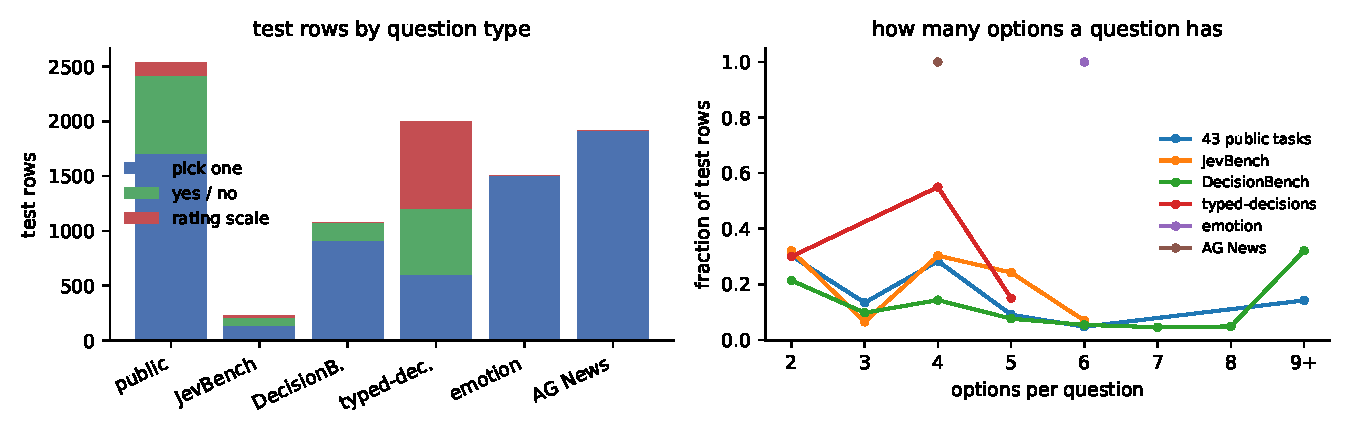
\includegraphics[width=\linewidth]{benchmarks.pdf}
\caption{Test-row distribution of the six benchmarks: question types (left) and number of options per question (right). DecisionBench and the public menu include questions with dozens to hundreds of options.}
\label{fig:bench}
\end{figure}

For DecisionBench we use the README's 1{,}075-row slice (25 rows per task, the notebook's seed) as the test set and a 100-per-task superset of the same tasks for feedback, as in our earlier DecisionBench study. For the public menu we use the harness's 60 evaluation rows per task and its 50 training rows per task as the feedback pool, the same 50 rows VegaML's TTT trains on. For typed-decisions we use the public LocalLLaMA release, which is what Laya reports on; Vega's README also quotes a typed-decisions number on six unpublished workflows that cannot be rerun.

\subsection{Protocol}
Every method learns only from feedback (or label) rows and is scored on the test rows; on JevBench, 5-fold cross-fitting keeps all paraphrases of a question in the same fold. The feedback rows of each task are split 80 / 20 into training and calibration rows with a fixed hash. All stochastic methods are run with seeds 0, 1, 2; we report mean $\pm$ s.d.\ over seeds. Gains are paired: the per-row correctness of a method (averaged over its seeds) minus that of the base model on the same rows, with a 95\% bootstrap CI over rows~\citep{efron1979bootstrap}, resampled within task for the macro-averaged public menu. Accuracy, ECE (15 equal-width bins, as in the README), NLL, skill, macro-F1, the JevBench tiers and paraphrase consistency, DecisionBench's domain slices and typed-decisions' soft accuracy all come from the harness's \texttt{score\_metrics}.

\subsection{Baselines}
\begin{itemize}
\item \textbf{Base model}: Vega 0.8B, Vega 4B, Laya, as released. Each is first \emph{replayed}: we re-run the frozen model on the cached inputs and check that its probabilities match the official prediction call (max absolute difference $\le 5\times10^{-5}$ for Laya, $0$ for Vega), and that its scores match the README.
\item \textbf{Their improvement, answer key}: for Vega, VegaML's TTT head (\texttt{fit()}, default settings) trained on the labelled feedback rows of each task; for Laya, the released \texttt{laya-typed-decisions} checkpoint, Laya's whole-model fine-tune on typed-decisions' labelled training split, scored on every benchmark.
\item \textbf{Answer-key add-on}: the same adapter (Vega) or head copy (Laya) trained with cross-entropy on the labels of the same rows and the same KL leash, then standard label-based temperature scaling on the same calibration rows. This is the upper bound \pk{} is measured against: same capacity, full information.
\item \textbf{\pk{}} and its ablations: no leash ($\beta = 0$), no honesty fix (the trained add-on with $T = 1$), with the switch, pooled, and on Laya the encoder-unfrozen variant.
\item \textbf{No-engine control} (DecisionBench study): a bilinear scorer on the same frozen features with the same feedback, leash and calibration, without Vega's engine.
\end{itemize}

\subsection{Compute and reproducibility}
The grid (6 benchmarks $\times$ 3 models $\times$ methods $\times$ 3 seeds, 233 steps) ran on one NVIDIA L40S in about five GPU-hours, from cached backbone features. One script, \texttt{experiments/peekaboo\_remaining/run.py}, runs every step, skips finished ones, retries failures and writes the tables; the results, logs and the table in this paper are in the repository.\footnote{\url{https://github.com/abhijithneilabraham/peekaboo}} All of Section~\ref{sec:curve} ran on a laptop CPU and was reproduced independently on a second machine (Appendix~\ref{app:repro}).

\section{Results}
\label{sec:results}

\subsection{Main comparison}

\begin{figure}[t]\centering
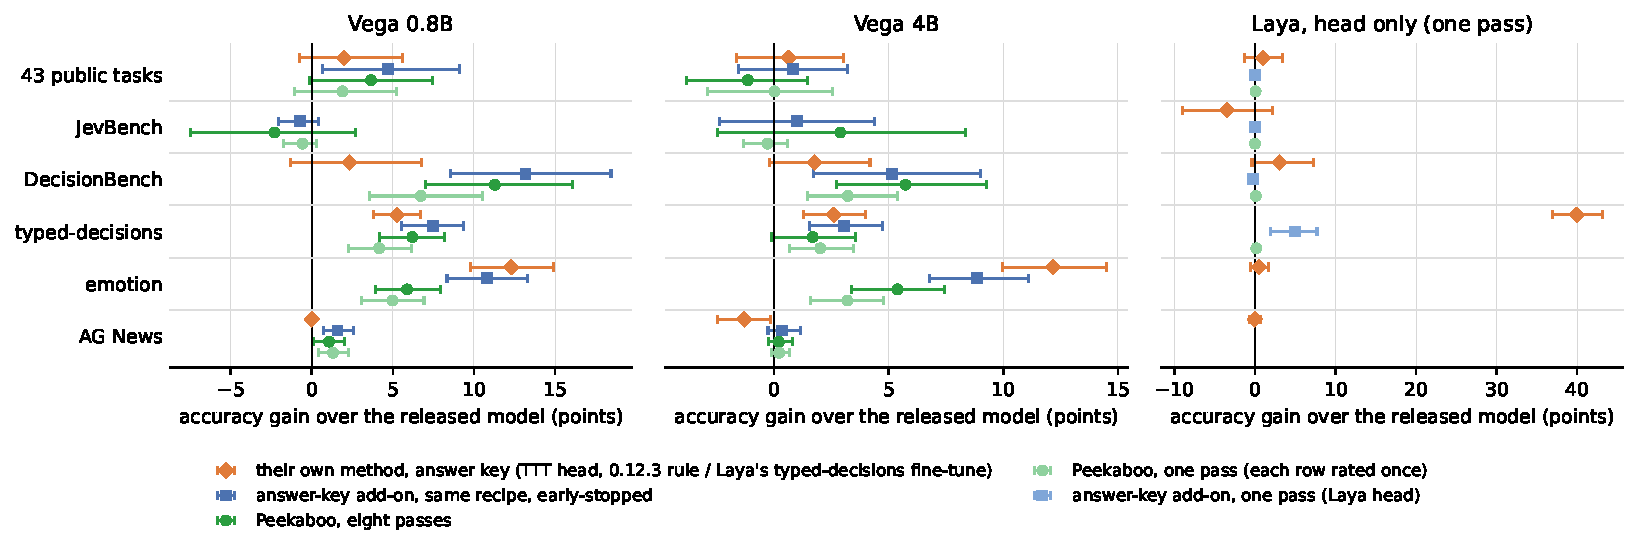
\includegraphics[width=\linewidth]{gains.pdf}
\caption{Accuracy gain over each base model on the six benchmarks (points; error bars are paired 95\% bootstrap CIs). Orange: the model's own answer-key improvement (VegaML's TTT head; Laya's released typed-decisions fine-tune). Blue: our add-on trained on the answer key. Greens: \pk{}, from right / wrong only.}
\label{fig:gains}
\end{figure}

% ---- acc
\begin{table}[tbp]\centering\scriptsize
\caption{Accuracy. Mean over 3 seeds ($\pm$ s.d.) where a method is stochastic. JevBench has no training split: Peekaboo learns by 5-fold cross-fitting (paraphrase groups kept together), pooled Peekaboo never sees it, and VegaML's TTT and the answer-key methods are not defined for it.}
\label{tab:acc}
\setlength{\tabcolsep}{2.5pt}
\begin{tabular}{llrrrrrrr}
\toprule
model & method & learns from & public & JevBench & DecisionB. & typed-dec. & emotion & AG News \\
\midrule
Vega 0.8B & base model & none & 0.556 & 0.550 & 0.509 & 0.665 & 0.568 & 0.901 \\
 & VegaML's TTT head & answer key & 0.533 & $\cdot$ & 0.531 & 0.721 & 0.638 & 0.897 \\
 & answer-key adapter & answer key & 0.584 {\scriptsize$\pm$0.005} & $\cdot$ & 0.628 {\scriptsize$\pm$0.008} & 0.734 {\scriptsize$\pm$0.000} & 0.630 {\scriptsize$\pm$0.011} & 0.907 {\scriptsize$\pm$0.001} \\
 & \textbf{Peekaboo} & right / wrong & 0.590 {\scriptsize$\pm$0.013} & 0.517 {\scriptsize$\pm$0.018} & 0.613 {\scriptsize$\pm$0.011} & 0.725 {\scriptsize$\pm$0.012} & 0.593 {\scriptsize$\pm$0.009} & 0.907 {\scriptsize$\pm$0.002} \\
 & pooled Peekaboo & right / wrong & 0.596 {\scriptsize$\pm$0.006} & 0.548 {\scriptsize$\pm$0.011} & 0.606 {\scriptsize$\pm$0.011} & 0.720 {\scriptsize$\pm$0.015} & 0.567 {\scriptsize$\pm$0.040} & 0.911 {\scriptsize$\pm$0.005} \\
\addlinespace
Vega 4B & base model & none & 0.715 & 0.667 & 0.631 & 0.730 & 0.579 & 0.927 \\
 & VegaML's TTT head & answer key & 0.677 & $\cdot$ & 0.639 & 0.753 & 0.651 & 0.919 \\
 & answer-key adapter & answer key & 0.705 {\scriptsize$\pm$0.005} & $\cdot$ & 0.683 {\scriptsize$\pm$0.011} & 0.774 {\scriptsize$\pm$0.006} & 0.592 {\scriptsize$\pm$0.022} & 0.921 {\scriptsize$\pm$0.003} \\
 & \textbf{Peekaboo} & right / wrong & 0.716 {\scriptsize$\pm$0.007} & 0.711 {\scriptsize$\pm$0.004} & 0.697 {\scriptsize$\pm$0.006} & 0.764 {\scriptsize$\pm$0.006} & 0.556 {\scriptsize$\pm$0.009} & 0.928 {\scriptsize$\pm$0.002} \\
 & pooled Peekaboo & right / wrong & 0.720 {\scriptsize$\pm$0.005} & 0.687 {\scriptsize$\pm$0.002} & 0.682 {\scriptsize$\pm$0.008} & 0.744 {\scriptsize$\pm$0.018} & 0.544 {\scriptsize$\pm$0.009} & 0.932 {\scriptsize$\pm$0.003} \\
\addlinespace
Laya & base model & none & 0.542 & 0.589 & 0.401 & 0.361 & 0.597 & 0.930 \\
 & laya-typed-decisions (Laya's fine-tune) & answer key & 0.551 & 0.537 & 0.438 & 0.762 & 0.604 & 0.930 \\
 & answer-key head & answer key & 0.535 {\scriptsize$\pm$0.004} & $\cdot$ & 0.389 {\scriptsize$\pm$0.009} & 0.544 {\scriptsize$\pm$0.005} & 0.540 {\scriptsize$\pm$0.032} & 0.930 {\scriptsize$\pm$0.000} \\
 & \textbf{Peekaboo}, head only & right / wrong & 0.543 {\scriptsize$\pm$0.001} & 0.584 {\scriptsize$\pm$0.000} & 0.405 {\scriptsize$\pm$0.002} & 0.493 {\scriptsize$\pm$0.008} & 0.596 {\scriptsize$\pm$0.001} & 0.930 {\scriptsize$\pm$0.000} \\
 & \textbf{Peekaboo}, encoder unfrozen & right / wrong & 0.572 {\scriptsize$\pm$0.007} & 0.558 {\scriptsize$\pm$0.011} & 0.559 {\scriptsize$\pm$0.005} & $\cdot$ & $\cdot$ & $\cdot$ \\
 & pooled Peekaboo, head only & right / wrong & 0.538 {\scriptsize$\pm$0.002} & 0.569 {\scriptsize$\pm$0.007} & 0.398 {\scriptsize$\pm$0.006} & 0.475 {\scriptsize$\pm$0.004} & 0.594 {\scriptsize$\pm$0.002} & 0.930 {\scriptsize$\pm$0.000} \\
\bottomrule
\end{tabular}
\end{table}

% ---- gain
\begin{table}[tbp]\centering\scriptsize
\caption{Gain over the base model, in accuracy points. Mean over 3 seeds ($\pm$ s.d.) where a method is stochastic. Each gain is paired on the same rows against the model's own base; the CIs are in Table~\ref{tab:h2h} and Figure~\ref{fig:gains}. JevBench has no training split: Peekaboo learns by 5-fold cross-fitting (paraphrase groups kept together), pooled Peekaboo never sees it, and VegaML's TTT and the answer-key methods are not defined for it.}
\label{tab:gain}
\setlength{\tabcolsep}{2.5pt}
\begin{tabular}{llrrrrrrr}
\toprule
model & method & learns from & public & JevBench & DecisionB. & typed-dec. & emotion & AG News \\
\midrule
Vega 0.8B & base model & none & -- & -- & -- & -- & -- & -- \\
 & VegaML's TTT head & answer key & -2.3 & $\cdot$ & +2.2 & +5.5 & +7.0 & -0.3 \\
 & answer-key adapter & answer key & +2.7 & $\cdot$ & +11.9 & +6.9 & +6.1 & +0.6 \\
 & \textbf{Peekaboo} & right / wrong & +3.4 & -3.3 & +10.4 & +5.9 & +2.5 & +0.7 \\
 & pooled Peekaboo & right / wrong & +4.0 & -0.1 & +9.7 & +5.4 & -0.2 & +1.1 \\
\addlinespace
Vega 4B & base model & none & -- & -- & -- & -- & -- & -- \\
 & VegaML's TTT head & answer key & -3.9 & $\cdot$ & +0.8 & +2.4 & +7.3 & -0.8 \\
 & answer-key adapter & answer key & -1.0 & $\cdot$ & +5.2 & +4.5 & +1.3 & -0.5 \\
 & \textbf{Peekaboo} & right / wrong & +0.1 & +4.5 & +6.7 & +3.4 & -2.3 & +0.1 \\
 & pooled Peekaboo & right / wrong & +0.4 & +2.0 & +5.1 & +1.4 & -3.5 & +0.5 \\
\addlinespace
Laya & base model & none & -- & -- & -- & -- & -- & -- \\
 & laya-typed-decisions (Laya's fine-tune) & answer key & +0.9 & -5.2 & +3.7 & +40.2 & +0.7 & +0.0 \\
 & answer-key head & answer key & -0.7 & $\cdot$ & -1.2 & +18.3 & -5.6 & +0.0 \\
 & \textbf{Peekaboo}, head only & right / wrong & +0.1 & -0.4 & +0.4 & +13.2 & -0.1 & +0.0 \\
 & \textbf{Peekaboo}, encoder unfrozen & right / wrong & +3.0 & -3.0 & +15.8 & $\cdot$ & $\cdot$ & $\cdot$ \\
 & pooled Peekaboo, head only & right / wrong & -0.4 & -2.0 & -0.2 & +11.4 & -0.2 & +0.0 \\
\bottomrule
\end{tabular}
\end{table}

% ---- ece
\begin{table}[tbp]\centering\scriptsize
\caption{Expected calibration error (lower is better). Mean over 3 seeds ($\pm$ s.d.) where a method is stochastic. JevBench has no training split: Peekaboo learns by 5-fold cross-fitting (paraphrase groups kept together), pooled Peekaboo never sees it, and VegaML's TTT and the answer-key methods are not defined for it.}
\label{tab:ece}
\setlength{\tabcolsep}{2.5pt}
\begin{tabular}{llrrrrrrr}
\toprule
model & method & learns from & public & JevBench & DecisionB. & typed-dec. & emotion & AG News \\
\midrule
Vega 0.8B & base model & none & 0.154 & 0.173 & 0.105 & 0.063 & 0.033 & 0.021 \\
 & VegaML's TTT head & answer key & 0.208 & $\cdot$ & 0.113 & 0.139 & 0.039 & 0.043 \\
 & answer-key adapter & answer key & 0.182 {\scriptsize$\pm$0.003} & $\cdot$ & 0.071 {\scriptsize$\pm$0.014} & 0.079 {\scriptsize$\pm$0.008} & 0.059 {\scriptsize$\pm$0.013} & 0.022 {\scriptsize$\pm$0.004} \\
 & \textbf{Peekaboo} & right / wrong & 0.203 {\scriptsize$\pm$0.007} & 0.092 {\scriptsize$\pm$0.018} & 0.055 {\scriptsize$\pm$0.015} & 0.077 {\scriptsize$\pm$0.019} & 0.070 {\scriptsize$\pm$0.025} & 0.016 {\scriptsize$\pm$0.004} \\
 & pooled Peekaboo & right / wrong & 0.193 {\scriptsize$\pm$0.024} & 0.108 {\scriptsize$\pm$0.034} & 0.066 {\scriptsize$\pm$0.009} & 0.062 {\scriptsize$\pm$0.031} & 0.068 {\scriptsize$\pm$0.023} & 0.019 {\scriptsize$\pm$0.005} \\
\addlinespace
Vega 4B & base model & none & 0.141 & 0.158 & 0.099 & 0.050 & 0.054 & 0.027 \\
 & VegaML's TTT head & answer key & 0.173 & $\cdot$ & 0.112 & 0.119 & 0.043 & 0.041 \\
 & answer-key adapter & answer key & 0.181 {\scriptsize$\pm$0.006} & $\cdot$ & 0.051 {\scriptsize$\pm$0.009} & 0.056 {\scriptsize$\pm$0.007} & 0.038 {\scriptsize$\pm$0.010} & 0.014 {\scriptsize$\pm$0.001} \\
 & \textbf{Peekaboo} & right / wrong & 0.172 {\scriptsize$\pm$0.003} & 0.098 {\scriptsize$\pm$0.008} & 0.049 {\scriptsize$\pm$0.009} & 0.044 {\scriptsize$\pm$0.013} & 0.035 {\scriptsize$\pm$0.012} & 0.018 {\scriptsize$\pm$0.003} \\
 & pooled Peekaboo & right / wrong & 0.176 {\scriptsize$\pm$0.015} & 0.134 {\scriptsize$\pm$0.038} & 0.057 {\scriptsize$\pm$0.019} & 0.050 {\scriptsize$\pm$0.005} & 0.044 {\scriptsize$\pm$0.009} & 0.016 {\scriptsize$\pm$0.006} \\
\addlinespace
Laya & base model & none & 0.212 & 0.113 & 0.174 & 0.183 & 0.306 & 0.012 \\
 & laya-typed-decisions (Laya's fine-tune) & answer key & 0.166 & 0.101 & 0.045 & 0.206 & 0.185 & 0.106 \\
 & answer-key head & answer key & 0.143 {\scriptsize$\pm$0.001} & $\cdot$ & 0.066 {\scriptsize$\pm$0.006} & 0.035 {\scriptsize$\pm$0.008} & 0.072 {\scriptsize$\pm$0.016} & 0.010 {\scriptsize$\pm$0.002} \\
 & \textbf{Peekaboo}, head only & right / wrong & 0.157 {\scriptsize$\pm$0.004} & 0.063 {\scriptsize$\pm$0.012} & 0.071 {\scriptsize$\pm$0.006} & 0.052 {\scriptsize$\pm$0.005} & 0.086 {\scriptsize$\pm$0.014} & 0.018 {\scriptsize$\pm$0.004} \\
 & \textbf{Peekaboo}, encoder unfrozen & right / wrong & 0.152 {\scriptsize$\pm$0.006} & 0.087 {\scriptsize$\pm$0.012} & 0.062 {\scriptsize$\pm$0.009} & $\cdot$ & $\cdot$ & $\cdot$ \\
 & pooled Peekaboo, head only & right / wrong & 0.164 {\scriptsize$\pm$0.007} & 0.096 {\scriptsize$\pm$0.019} & 0.067 {\scriptsize$\pm$0.015} & 0.052 {\scriptsize$\pm$0.016} & 0.087 {\scriptsize$\pm$0.006} & 0.016 {\scriptsize$\pm$0.003} \\
\bottomrule
\end{tabular}
\end{table}


\begin{table}[tbp]\centering\scriptsize
\caption{Head to head, in accuracy points with 95\% intervals (seeds and row clusters resampled). Positive means the first method is better. $\dagger$: survives Holm adjustment within the row's family; NI: non-inferior at a 2-point margin (lower bound above $-2$). TTT is scored under the vegaml 0.12.3 rule; for Laya ``their method'' is the typed-decisions fine-tune, in-domain only on typed-decisions.}
\label{tab:h2h}
\setlength{\tabcolsep}{3pt}
\resizebox{\linewidth}{!}{\begin{tabular}{llrrrrrr}
\toprule
model & comparison & public & JevBench & DecisionB. & typed-dec. & emotion & AG News \\
\midrule
\multicolumn{8}{l}{\textit{Vega 0.8B}} \\
 & Peekaboo (8 passes) vs. their method & +1.7 {\scriptsize[-1.6, +5.0]} & -- & +9.0 {\scriptsize[+5.4, +12.6]} & +0.9 {\scriptsize[-0.7, +2.7]} & -6.4 {\scriptsize[-8.4, -4.3]} & +1.1 {\scriptsize[+0.1, +2.0]} \\
 & Peekaboo (8) vs. answer key, same recipe (8) & +0.3 {\scriptsize[-2.8, +3.6]} & -1.4 {\scriptsize[-6.1, +3.0]} & -1.0 {\scriptsize[-3.0, +1.0]} & -0.9 {\scriptsize[-2.2, +0.5]} & -5.2 {\scriptsize[-7.1, -3.3]}$^{\dagger}$ & +1.0 {\scriptsize[-0.1, +2.1]} NI \\
 & Peekaboo (8) vs. answer key, early-stopped & -1.1 {\scriptsize[-4.0, +2.0]} & -1.6 {\scriptsize[-7.0, +3.5]} & -1.9 {\scriptsize[-4.1, +0.3]} & -1.3 {\scriptsize[-2.6, +0.1]} & -4.9 {\scriptsize[-6.8, -3.0]} & -0.5 {\scriptsize[-1.3, +0.2]} NI \\
 & Peekaboo (1 pass) vs. answer key (1 pass) & -1.7 {\scriptsize[-3.7, +0.5]} & -0.0 {\scriptsize[-1.0, +1.0]} NI & -3.2 {\scriptsize[-5.8, -0.6]} & -2.7 {\scriptsize[-4.1, -1.2]} & -1.7 {\scriptsize[-3.0, -0.4]} & -0.3 {\scriptsize[-0.9, +0.4]} NI \\
 & Peekaboo, 1 pass vs. 8 passes & -1.8 {\scriptsize[-4.4, +0.8]} & +1.7 {\scriptsize[-3.2, +7.2]} & -4.6 {\scriptsize[-8.1, -1.4]} & -2.1 {\scriptsize[-3.6, -0.4]} & -0.9 {\scriptsize[-2.4, +0.5]} & +0.2 {\scriptsize[-0.5, +1.0]} \\
 & logged best answers vs. Peekaboo (1 pass) & -- & -- & +0.7 {\scriptsize[-2.4, +3.7]} & +1.9 {\scriptsize[+0.3, +3.5]} NI & -1.5 {\scriptsize[-4.1, +0.7]} & -- \\
 & KL term vs. none & +1.1 {\scriptsize[-1.5, +3.9]} & +0.6 {\scriptsize[-2.4, +3.7]} & +1.2 {\scriptsize[-0.6, +3.0]} & +1.9 {\scriptsize[+0.3, +3.5]} & +0.5 {\scriptsize[-1.0, +1.8]} & -0.5 {\scriptsize[-1.3, +0.3]} \\
 & with the switch vs. without & +0.0 {\scriptsize[-2.2, +2.3]} & +2.3 {\scriptsize[-2.9, +7.7]} & +0.0 {\scriptsize[-1.2, +1.1]} & +0.0 {\scriptsize[-1.2, +1.3]} & +0.0 {\scriptsize[-1.1, +1.1]} & +0.0 {\scriptsize[-0.7, +0.7]} \\
\midrule
\multicolumn{8}{l}{\textit{Vega 4B}} \\
 & Peekaboo (8 passes) vs. their method & -1.8 {\scriptsize[-4.3, +0.7]} & -- & +4.0 {\scriptsize[+1.5, +6.5]} & -0.9 {\scriptsize[-2.6, +0.9]} & -6.8 {\scriptsize[-8.9, -4.7]} & +1.5 {\scriptsize[+0.4, +2.6]} \\
 & Peekaboo (8) vs. answer key, same recipe (8) & +0.0 {\scriptsize[-2.0, +2.0]} & -1.0 {\scriptsize[-5.0, +2.8]} & +0.6 {\scriptsize[-1.6, +2.7]} NI & -2.3 {\scriptsize[-3.8, -0.8]}$^{\dagger}$ & -1.1 {\scriptsize[-3.2, +1.0]} & +0.6 {\scriptsize[-0.1, +1.3]} NI \\
 & Peekaboo (8) vs. answer key, early-stopped & -2.0 {\scriptsize[-4.0, -0.2]} & +1.9 {\scriptsize[-2.7, +6.6]} & +0.6 {\scriptsize[-1.2, +2.3]} NI & -1.4 {\scriptsize[-2.9, +0.4]} & -3.5 {\scriptsize[-5.3, -1.7]} & -0.1 {\scriptsize[-0.8, +0.5]} NI \\
 & Peekaboo (1 pass) vs. answer key (1 pass) & -0.5 {\scriptsize[-3.0, +1.4]} & -0.3 {\scriptsize[-1.4, +0.7]} NI & -1.4 {\scriptsize[-3.8, +0.8]} & -2.6 {\scriptsize[-4.0, -1.2]} & -2.5 {\scriptsize[-3.7, -1.2]} & -0.1 {\scriptsize[-0.7, +0.5]} NI \\
 & Peekaboo, 1 pass vs. 8 passes & +1.2 {\scriptsize[-1.3, +3.5]} & -3.2 {\scriptsize[-8.7, +2.4]} & -2.5 {\scriptsize[-5.8, +0.0]} & +0.3 {\scriptsize[-1.2, +1.9]} & -2.2 {\scriptsize[-3.8, -0.5]} & +0.0 {\scriptsize[-0.6, +0.5]} \\
 & logged best answers vs. Peekaboo (1 pass) & -- & -- & -1.4 {\scriptsize[-4.4, +1.9]} & +2.0 {\scriptsize[+0.7, +3.4]} NI & +0.4 {\scriptsize[-1.9, +2.6]} NI & -- \\
 & KL term vs. none & -0.6 {\scriptsize[-2.8, +1.4]} & +0.3 {\scriptsize[-3.1, +3.8]} & +2.2 {\scriptsize[+0.4, +4.2]} & +0.4 {\scriptsize[-1.5, +2.3]} & +11.0 {\scriptsize[+8.5, +13.5]}$^{\dagger}$ & +0.2 {\scriptsize[-0.2, +0.8]} \\
 & with the switch vs. without & +0.0 {\scriptsize[-1.3, +1.2]} & -2.7 {\scriptsize[-8.1, +2.5]} & +0.0 {\scriptsize[-1.1, +1.2]} & -0.7 {\scriptsize[-3.0, +1.5]} & +0.0 {\scriptsize[-1.5, +1.6]} & +0.0 {\scriptsize[-0.5, +0.4]} \\
\midrule
\multicolumn{8}{l}{\textit{Laya}} \\
 & Peekaboo, head (1) vs. answer-key head (1) & +0.0 {\scriptsize[-0.3, +0.3]} NI & +0.0 {\scriptsize[+0.0, +0.0]} NI & +0.4 {\scriptsize[+0.1, +0.7]} NI & -4.8 {\scriptsize[-7.5, -2.0]} & -- & -- \\
 & Peekaboo, encoder (8) vs. their fine-tune & +1.6 {\scriptsize[-2.1, +5.3]} & +1.7 {\scriptsize[-4.7, +8.8]} & +10.9 {\scriptsize[+4.7, +16.7]}$^{\dagger}$ & -7.6 {\scriptsize[-9.8, -5.4]}$^{\dagger}$ & +21.6 {\scriptsize[+19.4, +24.0]}$^{\dagger}$ & -- \\
 & Peekaboo, encoder (8) vs. answer-key encoder, same recipe & -2.1 {\scriptsize[-5.1, +0.7]} & +2.3 {\scriptsize[-3.9, +7.9]} & -1.4 {\scriptsize[-5.1, +2.0]} & -6.5 {\scriptsize[-8.7, -4.1]}$^{\dagger}$ & -7.9 {\scriptsize[-9.6, -6.1]}$^{\dagger}$ & -- \\
 & Peekaboo, encoder (8) vs. answer-key encoder, early-stopped & -1.8 {\scriptsize[-4.7, +0.9]} & -3.6 {\scriptsize[-8.7, +1.4]} & -0.9 {\scriptsize[-4.5, +2.0]} & -6.5 {\scriptsize[-8.7, -4.3]} & -8.4 {\scriptsize[-10.2, -6.7]} & -- \\
 & Peekaboo, encoder: 1 pass vs. 8 & -0.4 {\scriptsize[-3.0, +2.1]} & +1.4 {\scriptsize[-4.4, +6.9]} & -6.3 {\scriptsize[-11.1, -1.9]} & -9.7 {\scriptsize[-12.1, -7.1]} & -12.2 {\scriptsize[-14.2, -10.3]} & -- \\
\bottomrule
\end{tabular}}
\end{table}


Table~\ref{tab:gain} and Figure~\ref{fig:gains} give the headline comparison; Table~\ref{tab:acc} the absolute accuracies and Table~\ref{tab:ece} the calibration errors. Three things stand out.

\paragraph{\pk{} beats Vega's own answer-key method on four of six benchmarks, at both sizes.}
On DecisionBench, \pk{} gains $+10.4$ [$+8.0$, $+12.8$] at 0.8B and $+6.7$ [$+4.6$, $+8.8$] at 4B, where VegaML's TTT head gains $+2.2$ and $+0.8$ with the labels. On the public menu \pk{} gains $+3.4$ and $+0.1$ while TTT \emph{loses} $2.3$ and $3.9$ points: the per-task head is fitted to 50 labelled rows and overturns Vega's zero-shot answer on tasks where it should not. On typed-decisions \pk{} and TTT are close at 0.8B ($+5.9$ vs.\ $+5.5$) and \pk{} is ahead at 4B ($+3.4$ vs.\ $+2.4$); on AG News both are within a point of base. TTT wins clearly on emotion ($+7.0$ / $+7.3$ vs.\ $+2.5$ / $-2.3$): a six-way single-label task with 4{,}000 labelled rows is exactly where a logistic-regression head on good features shines, and one bit per row is a poor substitute for the full label there.

\paragraph{\pk{} is within one to two points of training the same add-on on the answer key.}
The answer-key adapter is the information-rich upper bound with identical capacity. The paired difference \pk{} $-$ adapter is $+0.7$ [$-0.9$, $+2.2$] (public), $-1.5$ [$-3.5$, $+0.5$] (DecisionBench), $-0.9$ [$-2.5$, $+0.6$] (typed-decisions) and $+0.1$ (AG News) at 0.8B, and $+1.1$, $+1.5$, $-1.1$, $+0.6$ at 4B (Table~\ref{tab:h2h}); only emotion shows a clear gap ($-3.6$ / $-3.6$). The cheap signal buys most of what the expensive one does.

\paragraph{JevBench.}
JevBench is small (231 rows), has no training split and asks for judgment under paraphrase. \pk{} is the only method defined on it besides the base model (TTT and the answer-key methods need labelled training rows; the cross-fitted \pk{} uses rewards on the other folds). At 4B it is the only improvement we found: $+4.5$ [$+0.3$, $+9.0$]. At 0.8B it loses $3.3$ points [$-7.1$, $+0.4$]; the switch (Section~\ref{sec:ablation}) reduces that to $-0.6$ and pooling (Section~\ref{sec:pooled}) to $-0.1$.

\subsection{Calibration}

\begin{figure}[t]\centering
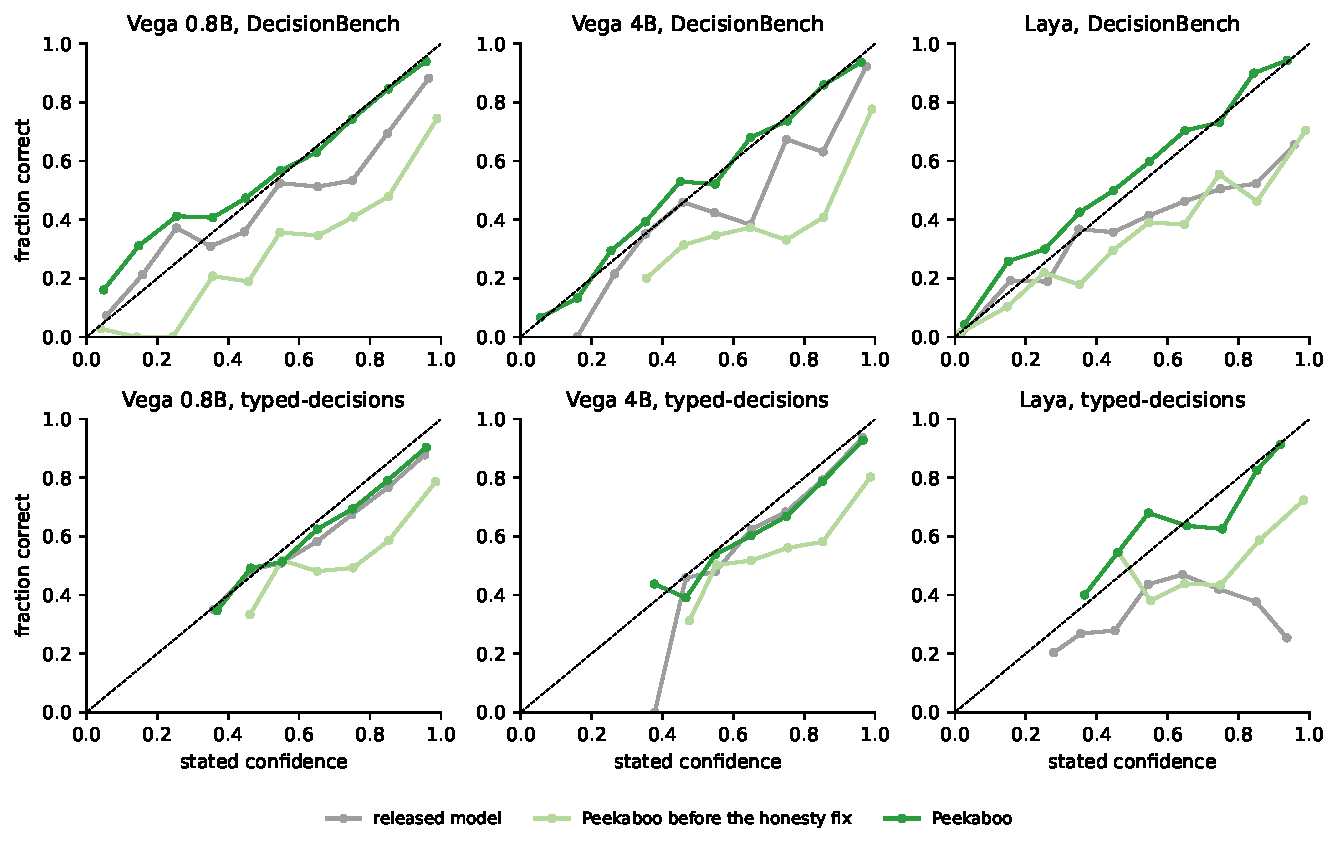
\includegraphics[width=0.9\linewidth]{reliability.pdf}
\caption{Reliability diagrams (10 bins on the confidence of the predicted option) on DecisionBench and typed-decisions. Grey: base model. Light green: the trained \pk{} add-on before the honesty fix, always over-confident. Dark green: \pk{}. The temperature fitted from right / wrong feedback puts the curves back on the diagonal.}
\label{fig:rel}
\end{figure}

Table~\ref{tab:ece} and Figure~\ref{fig:rel} show the calibration side. Policy-gradient training over-sharpens: without the honesty fix the add-on's ECE is 0.24 (DecisionBench, 0.8B), 0.22 (4B), 0.20 and 0.17 (typed-decisions). The feedback-fitted temperature brings these to 0.055, 0.049, 0.077 and 0.044, below the base model's 0.105, 0.099, 0.063 and 0.050 on DecisionBench and comparable on typed-decisions, and below the answer-key adapter with label-based temperature scaling on DecisionBench (0.071, 0.051). The exception is the public menu, where every trained method, \pk{} included, is worse calibrated than base Vega (0.203 vs.\ 0.154 at 0.8B): one temperature per benchmark is too coarse for 43 heterogeneous tasks whose option counts range from 2 to 151. On Laya the honesty fix is what makes the trained head usable at all: base Laya is poorly calibrated on DecisionBench (0.174) and emotion (0.306), and \pk{} brings both to 0.07--0.09.

\FloatBarrier
\subsection{Ablations}
\label{sec:ablation}
% ---- ablations
\begin{table}[tbp]\centering\scriptsize
\caption{Every variant and ablation: accuracy (top) and expected calibration error (bottom), mean over 3 seeds. ``switch'': the add-on is used only where held-out right / wrong feedback says it beats the base model. ``no honesty fix'': the trained add-on without the feedback-fitted temperature. ``KL 0'': no leash.}
\label{tab:ablation}
\setlength{\tabcolsep}{3pt}
\begin{tabular}{llrrrrrr}
\toprule
model & variant & public & JevBench & DecisionB. & typed-dec. & emotion & AG News \\
\midrule
\multicolumn{8}{l}{\textit{accuracy}} \\
\midrule
Vega 0.8B & base model & 0.556 & 0.550 & 0.509 & 0.665 & 0.568 & 0.901 \\
 & Peekaboo & 0.590 {\scriptsize$\pm$0.013} & 0.517 {\scriptsize$\pm$0.018} & 0.613 {\scriptsize$\pm$0.011} & 0.725 {\scriptsize$\pm$0.012} & 0.593 {\scriptsize$\pm$0.009} & 0.907 {\scriptsize$\pm$0.002} \\
 & Peekaboo + switch & 0.578 {\scriptsize$\pm$0.020} & 0.544 {\scriptsize$\pm$0.004} & 0.613 {\scriptsize$\pm$0.011} & 0.711 {\scriptsize$\pm$0.032} & 0.593 {\scriptsize$\pm$0.009} & 0.907 {\scriptsize$\pm$0.002} \\
 & Peekaboo without the honesty fix & 0.590 {\scriptsize$\pm$0.013} & 0.517 {\scriptsize$\pm$0.018} & 0.613 {\scriptsize$\pm$0.011} & 0.725 {\scriptsize$\pm$0.012} & 0.593 {\scriptsize$\pm$0.009} & 0.907 {\scriptsize$\pm$0.002} \\
 & Peekaboo without the leash (KL 0) & 0.568 {\scriptsize$\pm$0.021} & 0.509 {\scriptsize$\pm$0.025} & 0.612 {\scriptsize$\pm$0.007} & 0.698 {\scriptsize$\pm$0.020} & 0.529 {\scriptsize$\pm$0.020} & 0.908 {\scriptsize$\pm$0.001} \\
 & pooled Peekaboo (one add-on, all suites' feedback) & 0.596 {\scriptsize$\pm$0.006} & 0.548 {\scriptsize$\pm$0.011} & 0.606 {\scriptsize$\pm$0.011} & 0.720 {\scriptsize$\pm$0.015} & 0.567 {\scriptsize$\pm$0.040} & 0.911 {\scriptsize$\pm$0.005} \\
 & pooled Peekaboo + switch & 0.568 {\scriptsize$\pm$0.016} & 0.548 {\scriptsize$\pm$0.011} & 0.606 {\scriptsize$\pm$0.011} & 0.708 {\scriptsize$\pm$0.031} & 0.567 {\scriptsize$\pm$0.040} & 0.911 {\scriptsize$\pm$0.005} \\
 & pooled Peekaboo without the honesty fix & 0.596 {\scriptsize$\pm$0.006} & 0.548 {\scriptsize$\pm$0.011} & 0.606 {\scriptsize$\pm$0.011} & 0.720 {\scriptsize$\pm$0.015} & 0.567 {\scriptsize$\pm$0.040} & 0.911 {\scriptsize$\pm$0.005} \\
Vega 4B & base model & 0.715 & 0.667 & 0.631 & 0.730 & 0.579 & 0.927 \\
 & Peekaboo & 0.716 {\scriptsize$\pm$0.007} & 0.711 {\scriptsize$\pm$0.004} & 0.697 {\scriptsize$\pm$0.006} & 0.764 {\scriptsize$\pm$0.006} & 0.556 {\scriptsize$\pm$0.009} & 0.928 {\scriptsize$\pm$0.002} \\
 & Peekaboo + switch & 0.713 {\scriptsize$\pm$0.003} & 0.675 {\scriptsize$\pm$0.006} & 0.676 {\scriptsize$\pm$0.032} & 0.764 {\scriptsize$\pm$0.006} & 0.556 {\scriptsize$\pm$0.009} & 0.927 {\scriptsize$\pm$0.000} \\
 & Peekaboo without the honesty fix & 0.716 {\scriptsize$\pm$0.007} & 0.711 {\scriptsize$\pm$0.004} & 0.697 {\scriptsize$\pm$0.006} & 0.764 {\scriptsize$\pm$0.006} & 0.556 {\scriptsize$\pm$0.009} & 0.928 {\scriptsize$\pm$0.002} \\
 & Peekaboo without the leash (KL 0) & 0.707 {\scriptsize$\pm$0.008} & 0.704 {\scriptsize$\pm$0.011} & 0.681 {\scriptsize$\pm$0.002} & 0.741 {\scriptsize$\pm$0.007} & 0.521 {\scriptsize$\pm$0.022} & 0.930 {\scriptsize$\pm$0.002} \\
 & pooled Peekaboo (one add-on, all suites' feedback) & 0.720 {\scriptsize$\pm$0.005} & 0.687 {\scriptsize$\pm$0.002} & 0.682 {\scriptsize$\pm$0.008} & 0.744 {\scriptsize$\pm$0.018} & 0.544 {\scriptsize$\pm$0.009} & 0.932 {\scriptsize$\pm$0.003} \\
 & pooled Peekaboo + switch & 0.715 {\scriptsize$\pm$0.000} & 0.687 {\scriptsize$\pm$0.002} & 0.651 {\scriptsize$\pm$0.029} & 0.741 {\scriptsize$\pm$0.017} & 0.571 {\scriptsize$\pm$0.011} & 0.927 {\scriptsize$\pm$0.000} \\
 & pooled Peekaboo without the honesty fix & 0.720 {\scriptsize$\pm$0.005} & 0.687 {\scriptsize$\pm$0.002} & 0.682 {\scriptsize$\pm$0.008} & 0.744 {\scriptsize$\pm$0.018} & 0.544 {\scriptsize$\pm$0.009} & 0.932 {\scriptsize$\pm$0.003} \\
Laya & base model & 0.542 & 0.589 & 0.401 & 0.361 & 0.597 & 0.930 \\
 & Peekaboo & 0.543 {\scriptsize$\pm$0.001} & 0.584 {\scriptsize$\pm$0.000} & 0.405 {\scriptsize$\pm$0.002} & 0.493 {\scriptsize$\pm$0.008} & 0.596 {\scriptsize$\pm$0.001} & 0.930 {\scriptsize$\pm$0.000} \\
 & Peekaboo + switch & 0.542 {\scriptsize$\pm$0.000} & 0.586 {\scriptsize$\pm$0.002} & 0.401 {\scriptsize$\pm$0.000} & 0.493 {\scriptsize$\pm$0.008} & 0.597 {\scriptsize$\pm$0.000} & 0.930 {\scriptsize$\pm$0.000} \\
 & Peekaboo without the honesty fix & 0.543 {\scriptsize$\pm$0.001} & 0.584 {\scriptsize$\pm$0.000} & 0.405 {\scriptsize$\pm$0.002} & 0.493 {\scriptsize$\pm$0.008} & 0.596 {\scriptsize$\pm$0.001} & 0.930 {\scriptsize$\pm$0.000} \\
 & Peekaboo without the leash (KL 0) & 0.539 {\scriptsize$\pm$0.006} & 0.584 {\scriptsize$\pm$0.000} & 0.403 {\scriptsize$\pm$0.001} & 0.463 {\scriptsize$\pm$0.009} & 0.586 {\scriptsize$\pm$0.009} & 0.930 {\scriptsize$\pm$0.001} \\
 & Peekaboo, encoder unfrozen & 0.572 {\scriptsize$\pm$0.007} & 0.558 {\scriptsize$\pm$0.011} & 0.559 {\scriptsize$\pm$0.005} & $\cdot$ & $\cdot$ & $\cdot$ \\
 & Peekaboo, encoder unfrozen + switch & 0.555 {\scriptsize$\pm$0.019} & 0.579 {\scriptsize$\pm$0.017} & 0.559 {\scriptsize$\pm$0.005} & $\cdot$ & $\cdot$ & $\cdot$ \\
 & Peekaboo, encoder unfrozen, no honesty fix & 0.572 {\scriptsize$\pm$0.007} & 0.558 {\scriptsize$\pm$0.011} & 0.559 {\scriptsize$\pm$0.005} & $\cdot$ & $\cdot$ & $\cdot$ \\
 & pooled Peekaboo (one add-on, all suites' feedback) & 0.538 {\scriptsize$\pm$0.002} & 0.569 {\scriptsize$\pm$0.007} & 0.398 {\scriptsize$\pm$0.006} & 0.475 {\scriptsize$\pm$0.004} & 0.594 {\scriptsize$\pm$0.002} & 0.930 {\scriptsize$\pm$0.000} \\
 & pooled Peekaboo + switch & 0.542 {\scriptsize$\pm$0.000} & 0.569 {\scriptsize$\pm$0.007} & 0.401 {\scriptsize$\pm$0.000} & 0.475 {\scriptsize$\pm$0.004} & 0.597 {\scriptsize$\pm$0.000} & 0.930 {\scriptsize$\pm$0.000} \\
 & pooled Peekaboo without the honesty fix & 0.538 {\scriptsize$\pm$0.002} & 0.569 {\scriptsize$\pm$0.007} & 0.398 {\scriptsize$\pm$0.006} & 0.475 {\scriptsize$\pm$0.004} & 0.594 {\scriptsize$\pm$0.002} & 0.930 {\scriptsize$\pm$0.000} \\
\midrule
\multicolumn{8}{l}{\textit{calibration error (ECE)}} \\
\midrule
Vega 0.8B & base model & 0.154 & 0.173 & 0.105 & 0.063 & 0.033 & 0.021 \\
 & Peekaboo & 0.203 {\scriptsize$\pm$0.007} & 0.092 {\scriptsize$\pm$0.018} & 0.055 {\scriptsize$\pm$0.015} & 0.077 {\scriptsize$\pm$0.019} & 0.070 {\scriptsize$\pm$0.025} & 0.016 {\scriptsize$\pm$0.004} \\
 & Peekaboo + switch & 0.184 {\scriptsize$\pm$0.021} & 0.152 {\scriptsize$\pm$0.003} & 0.055 {\scriptsize$\pm$0.015} & 0.063 {\scriptsize$\pm$0.001} & 0.070 {\scriptsize$\pm$0.025} & 0.016 {\scriptsize$\pm$0.004} \\
 & Peekaboo without the honesty fix & 0.328 {\scriptsize$\pm$0.018} & 0.267 {\scriptsize$\pm$0.008} & 0.241 {\scriptsize$\pm$0.010} & 0.198 {\scriptsize$\pm$0.019} & 0.251 {\scriptsize$\pm$0.063} & 0.075 {\scriptsize$\pm$0.003} \\
 & Peekaboo without the leash (KL 0) & 0.213 {\scriptsize$\pm$0.016} & 0.097 {\scriptsize$\pm$0.014} & 0.082 {\scriptsize$\pm$0.024} & 0.052 {\scriptsize$\pm$0.006} & 0.048 {\scriptsize$\pm$0.009} & 0.018 {\scriptsize$\pm$0.003} \\
 & pooled Peekaboo (one add-on, all suites' feedback) & 0.193 {\scriptsize$\pm$0.024} & 0.108 {\scriptsize$\pm$0.034} & 0.066 {\scriptsize$\pm$0.009} & 0.062 {\scriptsize$\pm$0.031} & 0.068 {\scriptsize$\pm$0.023} & 0.019 {\scriptsize$\pm$0.005} \\
 & pooled Peekaboo + switch & 0.157 {\scriptsize$\pm$0.004} & 0.108 {\scriptsize$\pm$0.034} & 0.066 {\scriptsize$\pm$0.009} & 0.048 {\scriptsize$\pm$0.011} & 0.068 {\scriptsize$\pm$0.023} & 0.019 {\scriptsize$\pm$0.005} \\
 & pooled Peekaboo without the honesty fix & 0.267 {\scriptsize$\pm$0.038} & 0.308 {\scriptsize$\pm$0.022} & 0.232 {\scriptsize$\pm$0.051} & 0.154 {\scriptsize$\pm$0.018} & 0.311 {\scriptsize$\pm$0.110} & 0.073 {\scriptsize$\pm$0.014} \\
Vega 4B & base model & 0.141 & 0.158 & 0.099 & 0.050 & 0.054 & 0.027 \\
 & Peekaboo & 0.172 {\scriptsize$\pm$0.003} & 0.098 {\scriptsize$\pm$0.008} & 0.049 {\scriptsize$\pm$0.009} & 0.044 {\scriptsize$\pm$0.013} & 0.035 {\scriptsize$\pm$0.012} & 0.018 {\scriptsize$\pm$0.003} \\
 & Peekaboo + switch & 0.150 {\scriptsize$\pm$0.013} & 0.128 {\scriptsize$\pm$0.005} & 0.064 {\scriptsize$\pm$0.026} & 0.044 {\scriptsize$\pm$0.013} & 0.035 {\scriptsize$\pm$0.012} & 0.027 {\scriptsize$\pm$0.000} \\
 & Peekaboo without the honesty fix & 0.235 {\scriptsize$\pm$0.003} & 0.167 {\scriptsize$\pm$0.012} & 0.223 {\scriptsize$\pm$0.009} & 0.171 {\scriptsize$\pm$0.004} & 0.311 {\scriptsize$\pm$0.026} & 0.049 {\scriptsize$\pm$0.016} \\
 & Peekaboo without the leash (KL 0) & 0.182 {\scriptsize$\pm$0.011} & 0.099 {\scriptsize$\pm$0.005} & 0.075 {\scriptsize$\pm$0.027} & 0.049 {\scriptsize$\pm$0.016} & 0.052 {\scriptsize$\pm$0.004} & 0.016 {\scriptsize$\pm$0.002} \\
 & pooled Peekaboo (one add-on, all suites' feedback) & 0.176 {\scriptsize$\pm$0.015} & 0.134 {\scriptsize$\pm$0.038} & 0.057 {\scriptsize$\pm$0.019} & 0.050 {\scriptsize$\pm$0.005} & 0.044 {\scriptsize$\pm$0.009} & 0.016 {\scriptsize$\pm$0.006} \\
 & pooled Peekaboo + switch & 0.141 {\scriptsize$\pm$0.000} & 0.134 {\scriptsize$\pm$0.038} & 0.084 {\scriptsize$\pm$0.021} & 0.052 {\scriptsize$\pm$0.002} & 0.051 {\scriptsize$\pm$0.004} & 0.027 {\scriptsize$\pm$0.000} \\
 & pooled Peekaboo without the honesty fix & 0.227 {\scriptsize$\pm$0.020} & 0.261 {\scriptsize$\pm$0.024} & 0.253 {\scriptsize$\pm$0.027} & 0.202 {\scriptsize$\pm$0.013} & 0.321 {\scriptsize$\pm$0.006} & 0.056 {\scriptsize$\pm$0.005} \\
Laya & base model & 0.212 & 0.113 & 0.174 & 0.183 & 0.306 & 0.012 \\
 & Peekaboo & 0.157 {\scriptsize$\pm$0.004} & 0.063 {\scriptsize$\pm$0.012} & 0.071 {\scriptsize$\pm$0.006} & 0.052 {\scriptsize$\pm$0.005} & 0.086 {\scriptsize$\pm$0.014} & 0.018 {\scriptsize$\pm$0.004} \\
 & Peekaboo + switch & 0.212 {\scriptsize$\pm$0.000} & 0.084 {\scriptsize$\pm$0.007} & 0.174 {\scriptsize$\pm$0.000} & 0.052 {\scriptsize$\pm$0.005} & 0.306 {\scriptsize$\pm$0.000} & 0.015 {\scriptsize$\pm$0.005} \\
 & Peekaboo without the honesty fix & 0.319 {\scriptsize$\pm$0.009} & 0.228 {\scriptsize$\pm$0.002} & 0.329 {\scriptsize$\pm$0.027} & 0.351 {\scriptsize$\pm$0.014} & 0.347 {\scriptsize$\pm$0.012} & 0.059 {\scriptsize$\pm$0.000} \\
 & Peekaboo without the leash (KL 0) & 0.178 {\scriptsize$\pm$0.015} & 0.066 {\scriptsize$\pm$0.015} & 0.065 {\scriptsize$\pm$0.008} & 0.056 {\scriptsize$\pm$0.013} & 0.088 {\scriptsize$\pm$0.018} & 0.018 {\scriptsize$\pm$0.002} \\
 & Peekaboo, encoder unfrozen & 0.152 {\scriptsize$\pm$0.006} & 0.087 {\scriptsize$\pm$0.012} & 0.062 {\scriptsize$\pm$0.009} & $\cdot$ & $\cdot$ & $\cdot$ \\
 & Peekaboo, encoder unfrozen + switch & 0.189 {\scriptsize$\pm$0.033} & 0.092 {\scriptsize$\pm$0.012} & 0.062 {\scriptsize$\pm$0.009} & $\cdot$ & $\cdot$ & $\cdot$ \\
 & Peekaboo, encoder unfrozen, no honesty fix & 0.318 {\scriptsize$\pm$0.009} & 0.293 {\scriptsize$\pm$0.008} & 0.244 {\scriptsize$\pm$0.032} & $\cdot$ & $\cdot$ & $\cdot$ \\
 & pooled Peekaboo (one add-on, all suites' feedback) & 0.164 {\scriptsize$\pm$0.007} & 0.096 {\scriptsize$\pm$0.019} & 0.067 {\scriptsize$\pm$0.015} & 0.052 {\scriptsize$\pm$0.016} & 0.087 {\scriptsize$\pm$0.006} & 0.016 {\scriptsize$\pm$0.003} \\
 & pooled Peekaboo + switch & 0.212 {\scriptsize$\pm$0.000} & 0.096 {\scriptsize$\pm$0.019} & 0.174 {\scriptsize$\pm$0.000} & 0.052 {\scriptsize$\pm$0.016} & 0.306 {\scriptsize$\pm$0.000} & 0.012 {\scriptsize$\pm$0.000} \\
 & pooled Peekaboo without the honesty fix & 0.328 {\scriptsize$\pm$0.033} & 0.271 {\scriptsize$\pm$0.029} & 0.349 {\scriptsize$\pm$0.054} & 0.328 {\scriptsize$\pm$0.036} & 0.364 {\scriptsize$\pm$0.019} & 0.056 {\scriptsize$\pm$0.009} \\
\bottomrule
\end{tabular}
\end{table}



\begin{figure}[t]\centering
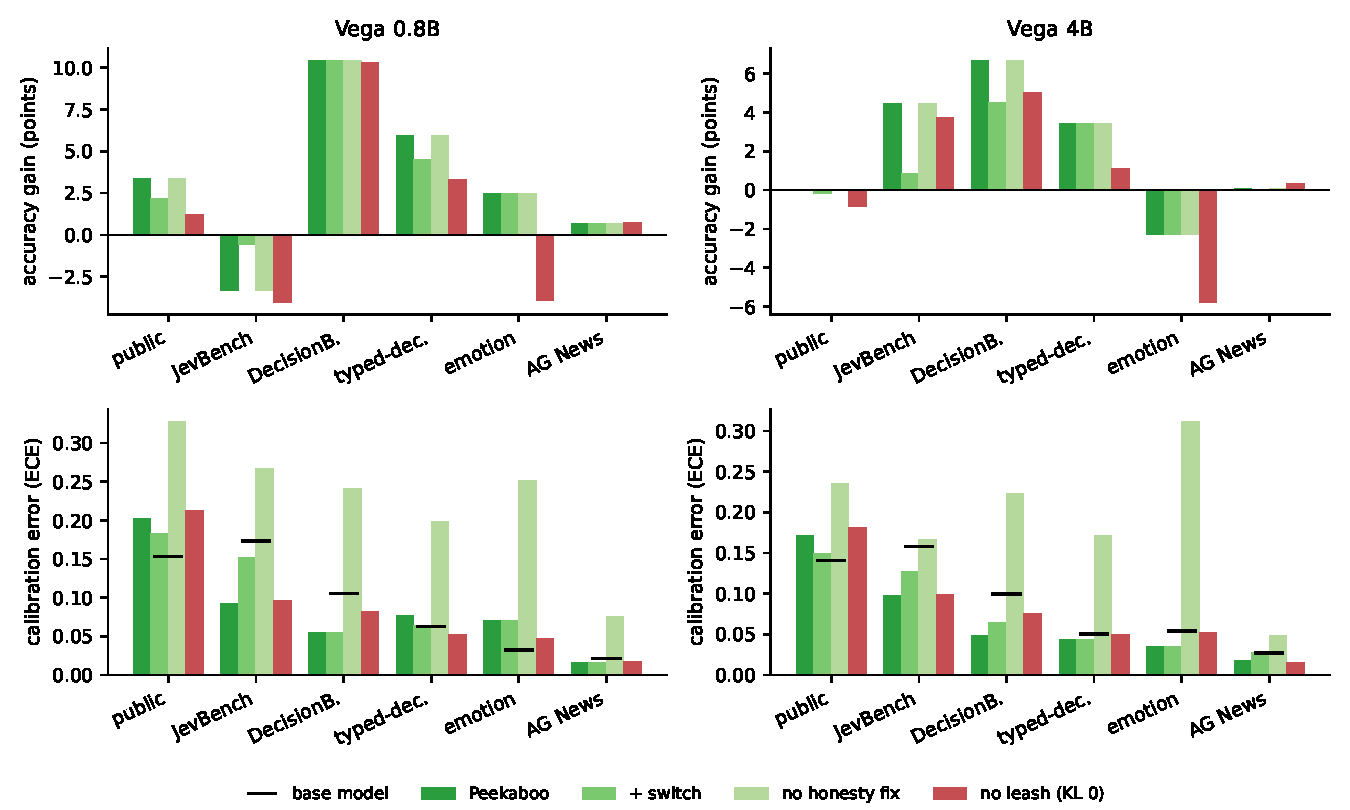
\includegraphics[width=0.9\linewidth]{ablation.pdf}
\caption{Ablations on Vega 0.8B (left) and 4B (right): accuracy gain (top) and ECE (bottom; black ticks are the base model). Removing the leash (KL 0) costs accuracy on five of six benchmarks; removing the honesty fix leaves accuracy unchanged but multiplies ECE; the switch trades gains for safety.}
\label{fig:ablation}
\end{figure}

Figure~\ref{fig:ablation} and Table~\ref{tab:ablation} isolate each part.

\paragraph{The leash.}
With $\beta = 0$ the gain drops on five of the six benchmarks at both sizes: at 0.8B from $+3.4$ to $+1.2$ (public), $-3.3$ to $-4.0$ (JevBench), $+5.9$ to $+3.3$ (typed-decisions) and $+2.5$ to $-3.9$ (emotion); at 4B from $+6.7$ to $+5.0$ (DecisionBench), $+3.4$ to $+1.1$ (typed-decisions) and $-2.3$ to $-5.8$ (emotion). Only AG News, where the base model is already at 0.90--0.93, is unaffected. The leash also keeps calibration closer to base on the public menu. In our earlier pilot a stronger leash ($\beta = 1$) was stable but kept only a third of the gain; $\beta = 0.1$ was chosen then and never retuned.

\paragraph{The honesty fix.}
By construction a temperature does not change the argmax, so accuracy is identical with and without it (Table~\ref{tab:ablation}); ECE is 1.6 to 4.4 times higher without it (public 0.203 $\to$ 0.328; DecisionBench 0.055 $\to$ 0.241; emotion 0.070 $\to$ 0.251 at 0.8B). Any system that uses the probabilities, for routing to a human or for conformal sets, needs this step.

\paragraph{The switch.}
The switch is a safety net, not a booster. It never turns a loss into a gain beyond base and sometimes removes a gain: at 4B it turns DecisionBench's $+6.7$ into $+4.5$ and JevBench's $+4.5$ into $+0.9$, because on a 42-row calibration fold a sampled comparison is noisy. Where \pk{} hurts, it helps: JevBench at 0.8B goes from $-3.3$ to $-0.6$ and the pooled add-on's emotion loss at 4B from $-3.5$ to $-0.8$. Figure~\ref{fig:switch_T} shows how often it fired; a deployment with more calibration rows than JevBench's 42 would get a more reliable switch.

\begin{figure}[t]\centering
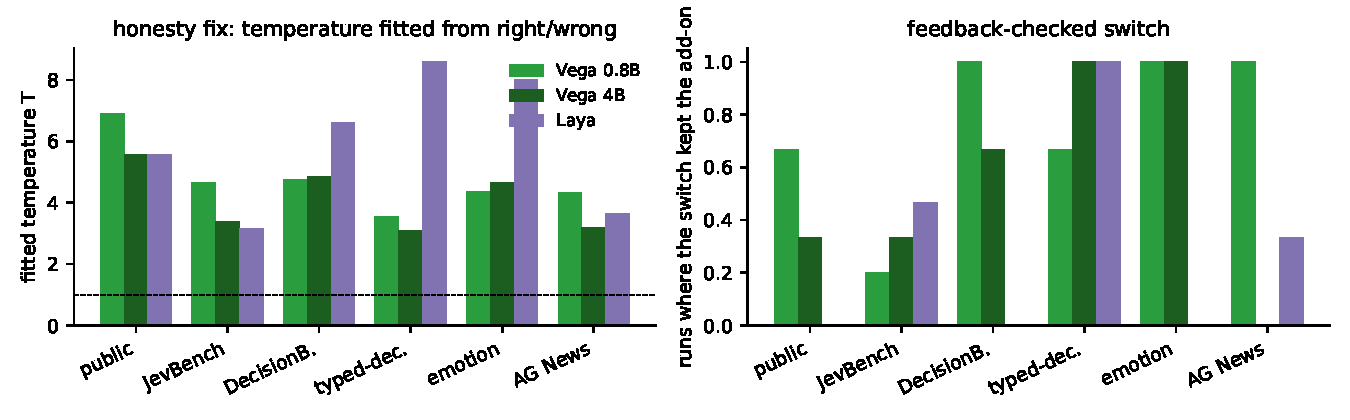
\includegraphics[width=0.9\linewidth]{switch_T.pdf}
\caption{Left: the temperature fitted from right / wrong feedback, per model and benchmark (dashed line: $T = 1$). Values of 3 to 9 show how much the trained policy had to be softened. Right: the fraction of runs in which the feedback-checked switch kept the add-on.}
\label{fig:switch_T}
\end{figure}

\subsection{Pooled \pk{}}
\label{sec:pooled}

\begin{figure}[t]\centering
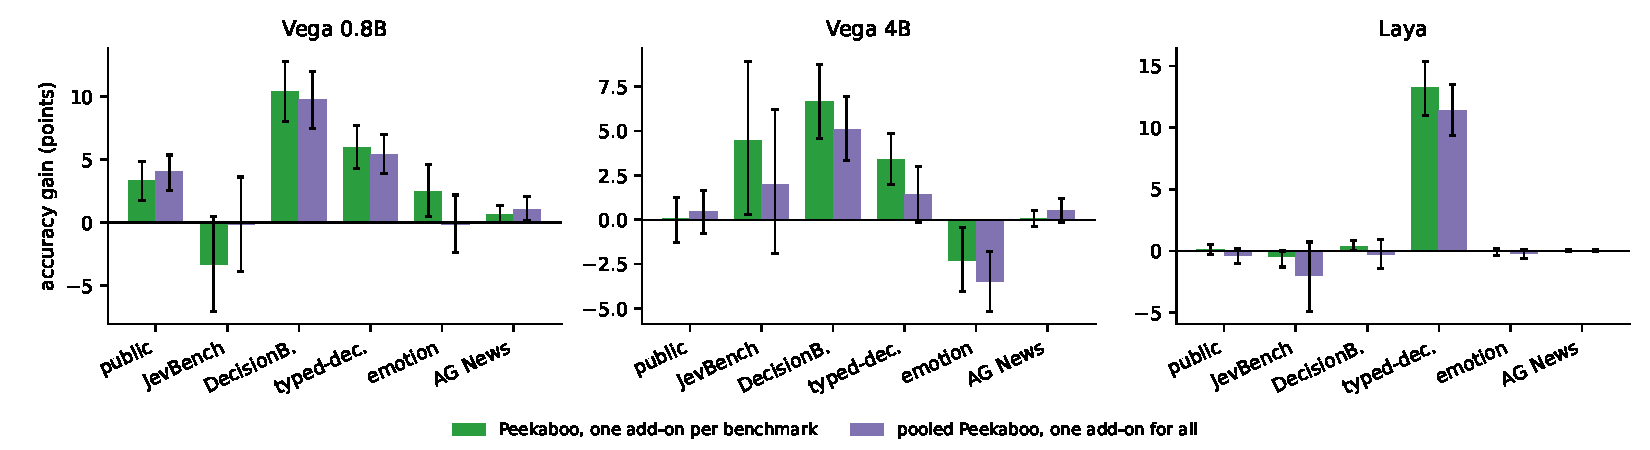
\includegraphics[width=\linewidth]{pooled.pdf}
\caption{One add-on per benchmark (green) against one pooled add-on trained on the feedback of all five benchmarks with a training split (purple). For the pooled add-on JevBench is pure transfer.}
\label{fig:pooled}
\end{figure}

One add-on trained on the feedback of every benchmark (Figure~\ref{fig:pooled}) is a mixed bag. At 0.8B it is slightly better on the public menu ($+4.0$ vs.\ $+3.4$) and AG News ($+1.1$ vs.\ $+0.7$), slightly worse on DecisionBench, typed-decisions and emotion, and it removes the JevBench loss ($-0.1$ vs.\ $-3.3$) although it never saw a JevBench row: feedback from 10{,}000 unrelated decisions teaches something general about how Vega mis-weighs options. At 4B, which already wins JevBench on its own, pooling is a little worse almost everywhere ($+2.0$ vs.\ $+4.5$ on JevBench, $+5.1$ vs.\ $+6.7$ on DecisionBench). On Laya's frozen-encoder head it is uniformly slightly worse. We therefore present pooling as an option for a model that must stay good on tasks it gets no feedback on, not as the default.

\FloatBarrier
\subsection{Laya: how much of the model \pk{} may change}
\label{sec:laya}
% ---- workflows
\begin{table}[tbp]\centering\small
\caption{typed-decisions accuracy per workflow (500 test decisions each).}
\label{tab:wf}
\setlength{\tabcolsep}{3pt}
\begin{tabular}{llrrrr}
\toprule
model & method & agent traces & customer service & invoices & security \\
\midrule
Vega 0.8B & base & 0.698 & 0.662 & 0.652 & 0.650 \\
 & TTT head & 0.690 & 0.716 & 0.800 & 0.678 \\
 & answer-key adapter & 0.703 & 0.743 & 0.805 & 0.687 \\
 & Peekaboo & 0.705 & 0.731 & 0.761 & 0.703 \\
\addlinespace
Vega 4B & base & 0.688 & 0.800 & 0.804 & 0.626 \\
 & TTT head & 0.700 & 0.800 & 0.808 & 0.706 \\
 & answer-key adapter & 0.707 & 0.813 & 0.815 & 0.763 \\
 & Peekaboo & 0.695 & 0.802 & 0.801 & 0.757 \\
\addlinespace
Laya & base & 0.388 & 0.380 & 0.360 & 0.316 \\
 & laya-typed-decisions & 0.732 & 0.766 & 0.810 & 0.742 \\
 & answer-key head & 0.507 & 0.501 & 0.619 & 0.551 \\
 & Peekaboo, head only & 0.437 & 0.473 & 0.535 & 0.528 \\
\bottomrule
\end{tabular}
\end{table}



\begin{figure}[t]\centering
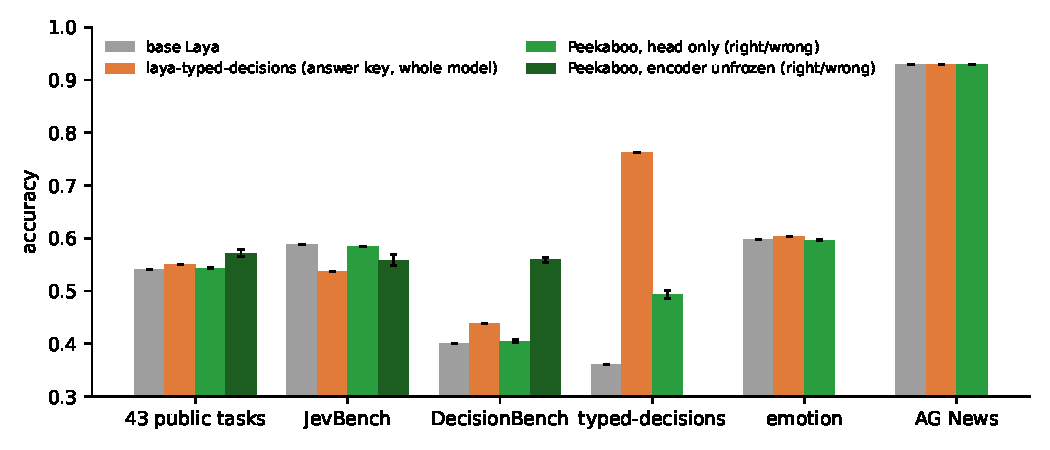
\includegraphics[width=0.85\linewidth]{laya.pdf}
\caption{Laya accuracy on the six benchmarks: base, Laya's released answer-key fine-tune of the whole model, \pk{} on the decision head alone, and \pk{} with the encoder unfrozen.}
\label{fig:laya}
\end{figure}

Laya's own improvement is a whole-model fine-tune on labels, and on its home benchmark it is very strong: typed-decisions goes from $0.361$ to $0.762$ ($+40.2$; the README says $0.766$). \pk{} on the frozen-encoder head gets $+13.2$ [$+11.0$, $+15.4$] from right / wrong alone, our answer-key head $+18.3$: the head is the bottleneck, not the signal. Unfreezing the encoder under the same right / wrong signal gives $\gainLayaEncTyped$ $\ciLayaEncTyped$ on typed-decisions (accuracy $\accLayaEncTyped$; Table~\ref{tab:h2h}, Figure~\ref{fig:laya}): more than the answer-key head, still short of the fine-tune's $+40.2$, which sees $\log_2 k$ bits per row where \pk{} sees one. Away from home the picture reverses. Laya's fine-tune loses $5.2$ points on JevBench and gains little elsewhere ($+0.9$ public, $+3.7$ DecisionBench), the classic cost of specialising a whole model; the head-only \pk{} changes nothing outside typed-decisions ($\pm 0.4$); and the encoder-unfrozen \pk{} gains $\gainLayaEncPub$ $\ciLayaEncPub$ on the public menu ($\accLayaEncPub$ vs.\ the fine-tune's $0.551$) and $\gainLayaEncDb$ $\ciLayaEncDb$ on DecisionBench ($\accLayaEncDb$ vs.\ $0.438$), $\gainLayaEncEmo$ $\ciLayaEncEmo$ on emotion ($\accLayaEncEmo$: the largest emotion result of any model or method in this paper, from right / wrong alone), with $\gainLayaEncJev$ on JevBench and $\gainLayaEncAg$ on AG News. Against the fine-tune directly it is $\gLayaEncVsTdPub$ (public), $\gLayaEncVsTdJev$ (JevBench), $\gLayaEncVsTdDb$ (DecisionBench) and $\gLayaEncVsTdTyped$ (typed-decisions) points. Table~\ref{tab:wf} breaks typed-decisions down by workflow.

\subsection{How much feedback, one pass, unseen tasks}
\label{sec:curve}

\begin{figure}[t]\centering
\begin{subfigure}{0.49\linewidth}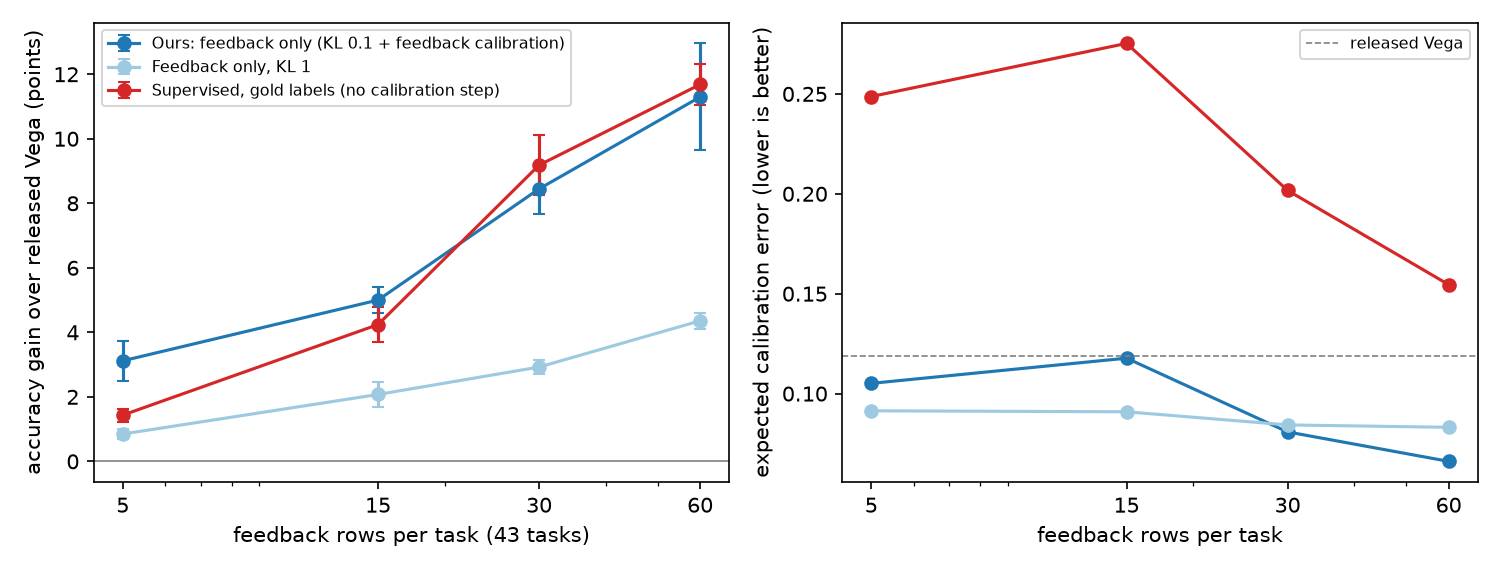
\includegraphics[width=\linewidth]{vega_feedback_curve.png}\caption{Vega 0.8B}\end{subfigure}\hfill
\begin{subfigure}{0.49\linewidth}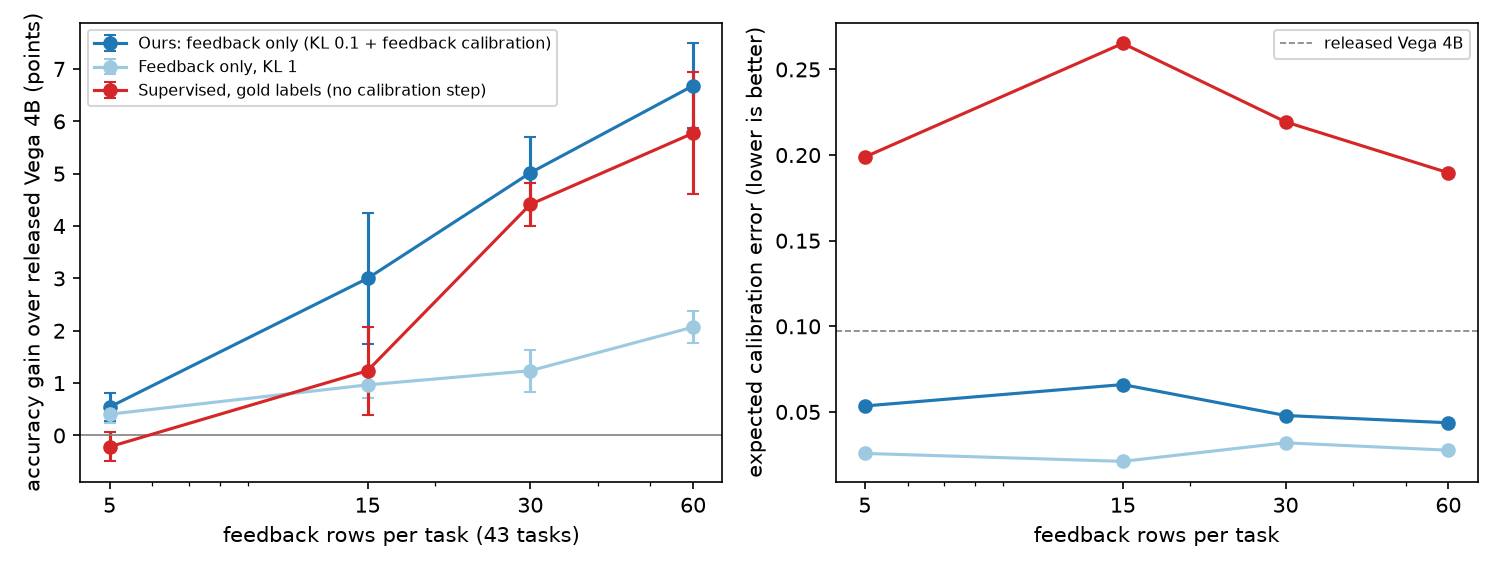
\includegraphics[width=\linewidth]{vega_feedback_curve_4b.png}\caption{Vega 4B}\end{subfigure}
\caption{DecisionBench, 1{,}720 held-out rows: accuracy gain (left of each panel) and ECE (right) against the number of feedback rows per task. Dashed: base model.}
\label{fig:curve}
\end{figure}

Our earlier DecisionBench study, which this grid extends, measured how the gain grows with feedback on a fixed 1{,}720-row test set (Figure~\ref{fig:curve}). At 0.8B the gain is $+3.1$, $+5.0$, $+8.4$ and $+11.3$ points with 5, 15, 30 and 60 feedback rows per task; at 4B, $+0.5$, $+3.0$, $+5.0$ and $+6.7$. From 15 rows per task on, feedback-only learning stays within about one point of label-supervised learning. Seeing each of the 2{,}560 rows exactly once, as in a live deployment, gives $+6.9$ (0.8B) and $+3.3$ (4B). Feedback on 33 tasks improves 10 tasks that gave none by $+4.2$ (0.8B) and $+4.6$ (4B) points. A no-engine control, the same feedback and leash on a bilinear scorer over the same frozen features, reaches only $0.26$ accuracy at either size: Vega's zero-shot energies are what make one bit per row enough.

\subsection{Reward during training}
Figure~\ref{fig:reward} shows the mean reward of the sampled answers over the eight passes. On Vega it rises steadily on every benchmark with a training split (DecisionBench 0.8B: 0.50 to 0.73); on Laya's frozen-encoder head it moves only on typed-decisions, consistent with the accuracy results. Since the sampled answer is right less often than the argmax, the reward curve also bounds the cost of exploration in a live system: on the first pass the policy is right about as often as the base model's samples, and better from the second pass on.

\begin{figure}[t]\centering
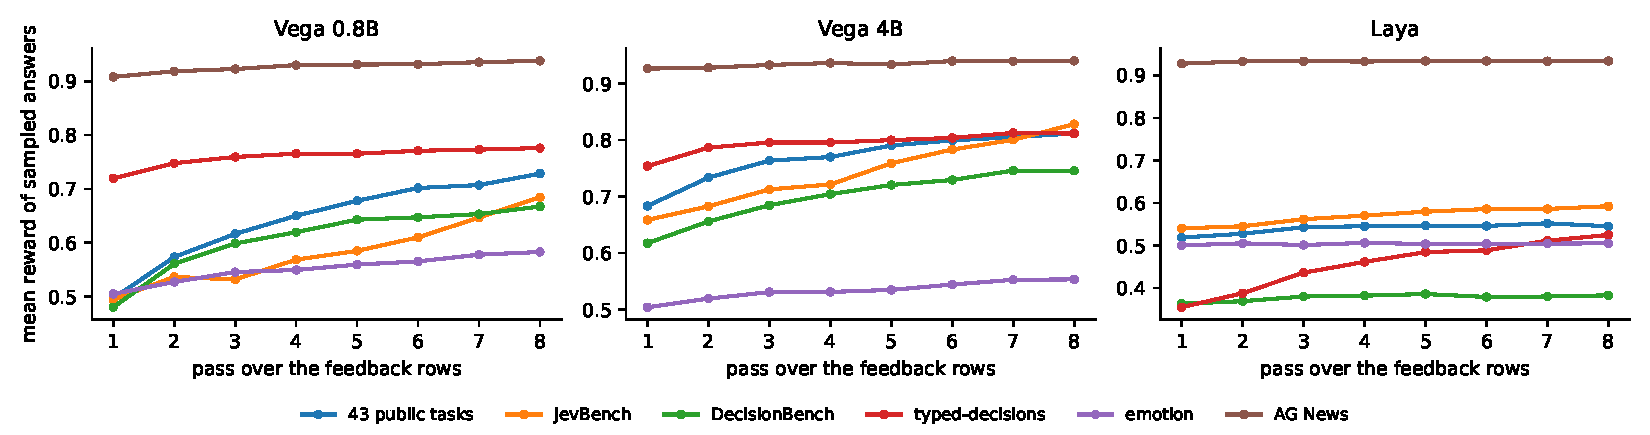
\includegraphics[width=\linewidth]{reward.pdf}
\caption{Mean reward of the sampled answers in each of the eight passes over the feedback rows (mean over seeds).}
\label{fig:reward}
\end{figure}

\FloatBarrier
\section{Discussion}

\paragraph{When \pk{} is the right tool.}
A model that is already deployed, collects right / wrong events as a by-product of use, and must stay good at everything it already does. There, with the same capacity, right / wrong recovers most of what the answer key would give (Section~\ref{sec:results}), the leash protects the rest, the switch guards against regressions, and the honesty fix keeps the probabilities usable. The gains are largest where the base model already leans towards the right option and mis-weighs it (DecisionBench's online-safety, home-automation and web domains in our earlier study), and smallest or negative where the task needs reasoning the base model lacks (DecisionBench's logic domain; JevBench's temporal-numeric family at 0.8B).

\paragraph{When it is not.}
A fixed task with thousands of fully labelled rows and permission to retrain the whole model. Laya's typed-decisions fine-tune ($+40$) is the clearest case; TTT on emotion for Vega is another. The answer key carries $\log_2 k$ bits per row against \pk{}'s one, and when the task is a clean single-label classification with many rows and the add-on is small, that difference shows. Give \pk{} more of the model, as in the Laya encoder-unfrozen runs, and one bit per row is enough even there: emotion rises from $0.597$ to $\accLayaEncEmo$ ($\gainLayaEncEmo$ points), where Laya's own fine-tune and VegaML's TTT reach $0.604$ and $0.651$ at best.

\paragraph{Why TTT loses on the public menu and DecisionBench.}
A TTT head is a per-task classifier with a fixed label set. Many DecisionBench rows have their own option list (a scale with different words per row, a list of candidate records), so \texttt{fit()} kept heads for 20 of the 43 tasks covering 394 of 1{,}075 rows and left the rest to the engine; \pk{} changes the engine, which reads the option text, so it applies to every row. On the public menu, 50 labelled rows per task are enough for a logistic head to overturn Vega's zero-shot answer on tasks where the zero-shot answer was better.

\section{Limitations}
\label{sec:limitations}
\begin{itemize}
\item \textbf{Simulated feedback.} The rewards are computed from gold answers: never wrong, never missing, never biased towards complaints. The method needs only a 0/1 signal, but we have not measured it under noisy, sparse or selective feedback. Our code has these settings (flip probability, report probability by outcome, logged off-policy feedback with clipped importance weights) and we leave their study to future work.
\item \textbf{Exploration has a cost.} During learning the model samples from its probabilities instead of taking the argmax; Figure~\ref{fig:reward} bounds the cost but we did not design a conservative exploration policy (e.g.\ exploring only inside Vega's conformal set).
\item \textbf{Hyper-parameters.} $\beta = 0.1$ was chosen in a pilot on parts of DecisionBench's 1{,}075 rows and never retuned; rank 8, 8 passes and learning rate $10^{-3}$ were fixed before any result. We did not tune TTT (VegaML defaults) or the answer-key add-on separately. Everything is reported with the same settings on all six benchmarks.
\item \textbf{One temperature per benchmark.} On the 43-task public menu this is too coarse; a per-task or per-option-count temperature, fitted the same way, is an obvious next step.
\item \textbf{Small benchmarks.} JevBench has 231 rows and 42-row calibration folds; its CIs are wide, and the switch is unreliable there.
\item \textbf{Vega's typed-decisions.} Vega's README reports typed-decisions on six unpublished workflows; we could only use Laya's public release, so Vega's own typed-decisions number is not directly compared.
\end{itemize}

\section{Conclusion}
A deployed decision model can improve from the one bit of feedback it actually receives. On the benchmarks Vega's and Laya's authors chose, a small add-on trained by REINFORCE on right / wrong rewards, held on a KL leash and re-calibrated with a temperature fitted from the same feedback, beats VegaML's own answer-key method on four of six benchmarks at both model sizes, matches an answer-key adapter of the same capacity within one to two points, and keeps or improves calibration. On Laya it is far behind a whole-model answer-key fine-tune on that model's home benchmark but does not pay that fine-tune's price elsewhere, and with the encoder unfrozen it overtakes the fine-tune on the public tasks and DecisionBench. The leash and the feedback-fitted temperature are both necessary, and a feedback-checked switch makes the add-on safe to turn on. Everything is reproducible from one script.

\paragraph{Acknowledgements.}
We thank the authors of VegaML and Laya for releasing their models, benchmark code and training recipes, which made a like-for-like comparison possible.

\FloatBarrier
\bibliographystyle{plainnat}
\bibliography{refs}

\appendix

\section{Reproducing the results}
\label{app:repro}
\texttt{experiments/peekaboo\_remaining/run.py} runs the entire grid: it reads every benchmark once through every model and caches the backbone features and the official records, replays each base model against its official prediction call, then runs every method and seed and writes \texttt{output/TABLES.md}, which is the source of every table here (via \texttt{paper/make\_figures.py}). Finished steps are skipped, so the run is resumable; failed steps are retried and listed in \texttt{output/STATUS.md}. \texttt{experiments/vega\_policy/reproduce.py} runs the DecisionBench study of Section~\ref{sec:curve} (feedback amount, one pass, unseen tasks, latency, the no-engine control and the Kuhn-poker~\citep{kuhn1950poker} experiment that started this work). A second person reproduced the 0.8B DecisionBench gain ($+10.4$ vs.\ our $+10.2$) and the released 4B accuracy ($0.635$ vs.\ the README's $0.633$) on a different machine before the grid was run.

\paragraph{Checks.} Replaying each frozen model on its cached inputs matches the official prediction call to $0$ (Vega) and $\le 5\times10^{-5}$ (Laya, one question per forward pass, as its own call runs, since padded batches move its probabilities by up to 0.02 under autocast). Base Vega 0.8B and 4B reproduce the README's public-menu accuracy ($0.556$ / $0.715$ vs.\ $0.556$ / $0.717$); base Laya and \texttt{laya-typed-decisions} reproduce the README's typed-decisions accuracy ($0.361$ / $0.762$ vs.\ $0.362$ / $0.766$).

\section{Per-task results on the public menu}
\label{app:tasks}
Table~\ref{tab:tasks} lists every public task. \pk{}'s largest gains over base Vega 0.8B are on prompt\_injections ($0.75 \to 0.87$), superglue\_cb ($0.67 \to 0.77$) and tweet\_sentiment ($0.44 \to 0.54$); its losses are on tasks where the TTT head also loses (unfair\_tos $0.74 \to 0.53$, TTT $0.63$; arc\_easy $0.60 \to 0.57$, TTT $0.35$). On Laya, the head-only add-on barely moves any task; the encoder-unfrozen variant lifts the safety tasks (aegis\_prompt\_safety $0.37 \to 0.69$, prompt\_injections $0.65 \to 0.78$) and the rating and topic tasks (yelp\_stars $0.28 \to 0.50$, trec\_coarse $0.53 \to 0.71$) while costing some intent tasks (banking77 $0.40 \to 0.33$).
\begin{table}[tbp]\centering\scriptsize
\caption{Accuracy on each of the 43 public tasks (mean over seeds). key: the early-stopped answer-key adapter / head; Pk8, Pk1: Peekaboo with eight passes, one pass; f-t: laya-typed-decisions; -enc: encoder unfrozen. $^*$ marks the two tasks with a construction artifact. Bold: the best method for that model on that task.}
\label{tab:tasks}
\setlength{\tabcolsep}{2pt}
\resizebox{\linewidth}{!}{\begin{tabular}{lrrrrrrrrrrrrrr}
\toprule
task & \multicolumn{5}{c}{Vega 0.8B} & \multicolumn{5}{c}{Vega 4B} & \multicolumn{4}{c}{Laya} \\
 & base & TTT & key & Pk8 & Pk1 & base & TTT & key & Pk8 & Pk1 & base & f-t & key-enc & Pk-enc \\
\midrule
aegis\_prompt\_safety & 0.50 & 0.50 & 0.64 & \textbf{0.64} & 0.57 & 0.60 & 0.60 & \textbf{0.79} & 0.74 & 0.73 & 0.37 & 0.43 & 0.68 & \textbf{0.70} \\
ag\_news & \textbf{0.97} & \textbf{0.97} & \textbf{0.97} & \textbf{0.97} & \textbf{0.97} & 0.95 & 0.95 & \textbf{0.97} & 0.95 & 0.97 & \textbf{0.98} & \textbf{0.98} & 0.97 & 0.97 \\
anli\_r3 & 0.28 & 0.28 & \textbf{0.39} & 0.37 & 0.32 & 0.35 & \textbf{0.52} & 0.43 & 0.40 & 0.39 & \textbf{0.43} & 0.40 & 0.42 & 0.42 \\
arc\_challenge & 0.48 & 0.48 & 0.44 & \textbf{0.50} & 0.48 & 0.80 & 0.80 & 0.80 & 0.81 & \textbf{0.83} & 0.28 & \textbf{0.37} & 0.34 & \textbf{0.37} \\
arc\_easy & \textbf{0.60} & \textbf{0.60} & 0.55 & 0.55 & 0.58 & 0.92 & 0.92 & \textbf{0.95} & 0.94 & 0.93 & 0.52 & 0.57 & \textbf{0.57} & 0.57 \\
banking77 & 0.68 & 0.68 & \textbf{0.72} & 0.66 & 0.62 & 0.73 & 0.73 & \textbf{0.74} & 0.69 & 0.69 & 0.42 & 0.40 & \textbf{0.48} & 0.37 \\
boolq & 0.75 & 0.75 & 0.76 & \textbf{0.82} & 0.79 & 0.82 & 0.82 & 0.84 & 0.84 & \textbf{0.91} & \textbf{0.87} & 0.85 & 0.78 & 0.83 \\
casehold & 0.35 & 0.35 & \textbf{0.49} & 0.46 & 0.42 & 0.55 & 0.55 & \textbf{0.63} & 0.61 & 0.63 & 0.38 & 0.38 & 0.38 & \textbf{0.45} \\
climate\_fever & 0.35 & 0.38 & \textbf{0.47} & 0.38 & 0.36 & 0.45 & 0.38 & \textbf{0.48} & 0.46 & \textbf{0.48} & 0.33 & \textbf{0.35} & 0.25 & 0.30 \\
clinc150\_oos & \textbf{0.68} & \textbf{0.68} & 0.62 & 0.62 & 0.61 & \textbf{0.92} & \textbf{0.92} & 0.83 & 0.78 & 0.83 & 0.00 & \textbf{0.32} & 0.00 & 0.00 \\
commonsenseqa & 0.35 & 0.35 & \textbf{0.41} & 0.38 & 0.35 & 0.53 & 0.53 & 0.59 & 0.59 & \textbf{0.60} & 0.45 & 0.45 & \textbf{0.47} & 0.45 \\
cruxeval\_output & 0.65 & 0.65 & \textbf{0.87} & 0.79 & 0.82 & 0.85 & 0.92 & \textbf{0.94} & 0.92 & \textbf{0.94} & 0.78 & 0.73 & 0.79 & \textbf{0.81} \\
dbpedia14 & 0.60 & \textbf{0.85} & 0.77 & 0.67 & 0.72 & 0.90 & \textbf{0.97} & 0.92 & 0.93 & 0.90 & 0.85 & 0.83 & 0.91 & \textbf{0.93} \\
emotion & \textbf{0.55} & \textbf{0.55} & 0.43 & 0.53 & 0.54 & \textbf{0.63} & 0.45 & 0.52 & 0.52 & 0.61 & \textbf{0.57} & \textbf{0.57} & 0.53 & 0.53 \\
enron\_spam & \textbf{1.00} & \textbf{1.00} & \textbf{1.00} & 0.99 & \textbf{1.00} & \textbf{1.00} & \textbf{1.00} & \textbf{1.00} & \textbf{1.00} & 0.99 & 0.92 & 0.90 & \textbf{0.93} & 0.92 \\
glue\_rte & \textbf{0.62} & \textbf{0.62} & 0.61 & \textbf{0.62} & 0.58 & 0.87 & 0.85 & 0.87 & 0.86 & \textbf{0.89} & \textbf{0.83} & 0.82 & 0.82 & 0.80 \\
hellaswag & 0.25 & 0.25 & 0.27 & \textbf{0.32} & 0.28 & \textbf{0.65} & \textbf{0.65} & 0.58 & 0.53 & 0.59 & 0.37 & 0.37 & 0.39 & \textbf{0.39} \\
jailbreak\_cls & \textbf{0.98} & \textbf{0.98} & \textbf{0.98} & 0.97 & 0.96 & \textbf{1.00} & \textbf{1.00} & 0.99 & 0.98 & 0.99 & 0.98 & 0.98 & 0.98 & \textbf{0.99} \\
ledgar & 0.33 & 0.33 & \textbf{0.59} & 0.40 & 0.39 & 0.63 & 0.63 & 0.63 & 0.63 & \textbf{0.66} & 0.25 & 0.18 & \textbf{0.47} & 0.33 \\
massive\_intent\_en & 0.38 & 0.38 & \textbf{0.53} & 0.43 & 0.43 & 0.60 & 0.60 & \textbf{0.64} & 0.59 & 0.60 & 0.38 & 0.42 & \textbf{0.47} & 0.38 \\
medmcqa & 0.18 & 0.18 & 0.19 & 0.28 & \textbf{0.30} & 0.48 & 0.48 & \textbf{0.49} & \textbf{0.49} & 0.48 & \textbf{0.35} & \textbf{0.35} & 0.32 & 0.31 \\
medqa\_usmle & 0.31 & 0.31 & 0.27 & 0.29 & \textbf{0.31} & 0.51 & 0.51 & \textbf{0.55} & 0.53 & \textbf{0.55} & 0.20 & \textbf{0.29} & 0.23 & 0.28 \\
mmlu & \textbf{0.37} & \textbf{0.37} & 0.32 & 0.32 & 0.31 & \textbf{0.73} & \textbf{0.73} & 0.63 & 0.57 & 0.61 & 0.25 & \textbf{0.35} & 0.31 & 0.32 \\
mmlu\_pro & 0.20 & 0.13 & 0.16 & 0.21 & \textbf{0.24} & \textbf{0.40} & \textbf{0.40} & 0.39 & \textbf{0.40} & 0.38 & \textbf{0.18} & \textbf{0.18} & \textbf{0.18} & 0.18 \\
openbookqa & \textbf{0.58} & \textbf{0.58} & 0.53 & 0.54 & 0.58 & \textbf{0.83} & \textbf{0.83} & 0.79 & 0.78 & 0.79 & 0.40 & 0.48 & \textbf{0.53} & 0.49 \\
prompt\_injections & 0.75 & \textbf{0.96} & 0.87 & 0.85 & 0.76 & 0.85 & \textbf{0.96} & 0.82 & 0.89 & 0.90 & 0.65 & 0.60 & 0.81 & \textbf{0.84} \\
pubmedqa$^*$ & 0.13 & \textbf{0.58} & 0.54 & 0.55 & 0.54 & 0.40 & \textbf{0.62} & 0.60 & 0.56 & 0.55 & 0.53 & 0.55 & \textbf{0.64} & 0.61 \\
race\_middle & 0.60 & 0.60 & 0.54 & \textbf{0.61} & 0.57 & 0.82 & \textbf{0.90} & 0.82 & 0.81 & 0.82 & 0.58 & 0.52 & \textbf{0.59} & 0.53 \\
sciq & 0.73 & 0.73 & 0.67 & 0.72 & \textbf{0.76} & 0.92 & 0.92 & \textbf{0.95} & 0.94 & 0.93 & 0.52 & 0.55 & \textbf{0.56} & 0.52 \\
superglue\_cb & 0.67 & 0.69 & 0.68 & \textbf{0.75} & 0.70 & 0.82 & \textbf{0.87} & 0.81 & 0.78 & 0.82 & \textbf{0.87} & 0.84 & 0.83 & 0.79 \\
toxic\_chat\_jailbreak & \textbf{0.98} & \textbf{0.98} & 0.96 & 0.91 & 0.92 & 0.92 & 0.92 & \textbf{0.95} & \textbf{0.95} & 0.94 & 0.83 & \textbf{0.90} & 0.84 & 0.87 \\
toxic\_chat\_toxicity & \textbf{0.95} & 0.93 & 0.93 & 0.90 & 0.92 & \textbf{1.00} & 0.98 & 0.98 & 0.98 & 0.98 & \textbf{0.97} & \textbf{0.97} & 0.94 & 0.92 \\
trec\_coarse & 0.53 & 0.68 & \textbf{0.72} & 0.61 & 0.60 & 0.77 & \textbf{0.88} & 0.83 & 0.77 & 0.75 & 0.57 & 0.52 & \textbf{0.89} & 0.56 \\
truthfulqa\_mc1$^*$ & 0.34 & 0.34 & \textbf{0.77} & 0.71 & 0.53 & 0.64 & 0.64 & \textbf{0.73} & 0.72 & 0.65 & 0.16 & 0.24 & \textbf{0.41} & 0.38 \\
tweet\_hate & \textbf{0.65} & 0.63 & 0.62 & 0.61 & 0.53 & \textbf{0.68} & 0.60 & 0.57 & 0.61 & 0.59 & \textbf{0.73} & 0.72 & 0.64 & 0.67 \\
tweet\_irony & \textbf{0.78} & 0.60 & 0.71 & 0.67 & 0.70 & \textbf{0.78} & \textbf{0.78} & 0.74 & 0.73 & 0.71 & \textbf{0.78} & 0.74 & 0.71 & 0.73 \\
tweet\_offensive & 0.80 & 0.80 & 0.81 & 0.80 & \textbf{0.81} & 0.78 & 0.78 & \textbf{0.85} & 0.78 & 0.80 & 0.69 & 0.71 & \textbf{0.79} & 0.78 \\
tweet\_sentiment & 0.44 & 0.44 & 0.45 & \textbf{0.50} & 0.46 & \textbf{0.58} & \textbf{0.58} & 0.49 & 0.56 & 0.49 & \textbf{0.56} & 0.49 & 0.45 & 0.45 \\
tweet\_stance\_abortion & 0.36 & 0.45 & 0.48 & \textbf{0.58} & 0.40 & \textbf{0.55} & 0.49 & 0.48 & 0.31 & 0.45 & 0.31 & 0.31 & 0.38 & \textbf{0.44} \\
unfair\_tos & \textbf{0.74} & 0.65 & 0.56 & 0.57 & 0.54 & \textbf{0.88} & 0.70 & 0.82 & 0.73 & 0.71 & \textbf{0.88} & 0.84 & 0.61 & 0.61 \\
vitaminc & 0.47 & 0.47 & \textbf{0.54} & 0.47 & 0.53 & 0.62 & 0.62 & 0.63 & 0.61 & \textbf{0.64} & 0.43 & 0.33 & \textbf{0.66} & 0.62 \\
winogrande & 0.50 & 0.50 & \textbf{0.52} & 0.49 & 0.51 & 0.58 & 0.58 & 0.62 & \textbf{0.63} & \textbf{0.63} & 0.53 & 0.50 & 0.53 & \textbf{0.57} \\
yelp\_stars & 0.50 & 0.50 & \textbf{0.59} & 0.49 & 0.45 & \textbf{0.58} & \textbf{0.58} & 0.52 & 0.47 & 0.52 & 0.28 & 0.37 & \textbf{0.59} & 0.38 \\
\bottomrule
\end{tabular}}
\end{table}

\FloatBarrier

\section{Hyper-parameters}
\begin{table}[H]\centering\small
\begin{tabular}{lp{12.5cm}}
\toprule
add-on, Vega & gated LoRA, rank 8, on the engine's input layers (\texttt{vegaml.attach\_adapter}); 409k / 857k parameters \\
add-on, Laya & trainable copy of type embedding, 2-layer decision head and scorer; encoder frozen, or a trained copy (``encoder unfrozen'') \\
optimiser & Adam; lr $10^{-3}$ (Vega adapter), $10^{-4}$ (Laya head), $2.5\times10^{-5}$ (Laya encoder); grad-norm clip 1.0 \\
schedule & 8 passes, batches of 32 (Laya encoder: micro-batches of 8, one update per 32 rows) \\
reward & $r = \mathbf{1}[\text{sampled answer} = \text{gold}]$; baseline $b \leftarrow 0.9\,b + 0.1\,\bar r$, $b_0 = 0.5$ \\
leash & $\beta = 0.1$ (ablation: 0) \\
honesty fix & $T$ on a 61-point log grid in $[0.25, 32]$, maximising the Bernoulli likelihood of right / wrong on the calibration rows \\
splits & feedback rows 80\,/\,20 train\,/\,calibration per task by a fixed hash; JevBench 5-fold by paraphrase group \\
seeds & 0, 1, 2 \\
\bottomrule
\end{tabular}
\end{table}

\end{document}
